\documentclass[a4paper,fontsize=13pt]{scrreprt}

\usepackage[francais]{babel}

\usepackage[utf8]{inputenc}
\usepackage[T1]{fontenc}
\usepackage{pifont}
%\usepackage{verdana}
\usepackage{ulem}

\usepackage{amsmath}
\usepackage{amssymb}
\usepackage{amsthm}
\usepackage{amscd}
\usepackage{mathabx}
\usepackage{hyperref}
\usepackage{setspace} 
\usepackage{multicol}
\onehalfspacing

\usepackage[abbrev,backrefs]{amsrefs}
\usepackage{eurosym}


\usepackage{graphicx}
\usepackage{array}

\usepackage[framemethod=TikZ]{mdframed} % Cadres
\usepackage{tikz}
\usepackage{tkz-euclide}
\usetkzobj{all}
\usepackage{tikz-3dplot}
\usetikzlibrary{calc,backgrounds}

\usepackage[all]{xy}
\usepackage{flowchart}
\usetikzlibrary{arrows}

\usepackage{geometry}
\geometry{hmargin=2.5cm,vmargin=2.5cm}
\pagestyle{myheadings}
\renewcommand{\chaptermark}[1]{\markboth{\textbf{\thechapter. #1}}{}}
\renewcommand{\sectionmark}[1]{\markright{\textbf{\thesection. #1}}}

\renewcommand{\familydefault}{\sfdefault}

\theoremstyle{plain}
\newtheorem{thé}[subsection]{Théorème}
\newtheorem*{thé*}{Théorème}
\newtheorem{pro}[subsection]{Proposition}
\newtheorem*{pro*}{Proposition}
\newtheorem{cor}[subsection]{Corollaire}	
\newtheorem*{cor*}{Corollaire}
\newtheorem{lem}[subsection]{Lemme}		

\theoremstyle{definition}
\newtheorem{déf}[subsection]{Définition}
\newtheorem{exe}[subsection]{Exemple}
\newtheorem{con}[subsection]{Contre-exemple}
\newtheorem{rema}[subsection]{Remarque}	
\newtheorem*{rema*}{Remarque}	
\newtheorem*{nota}{Notation}
\newtheorem*{prob}{Problème}	
\newtheorem*{epcs}{Exercices pour cette section}
\newtheorem{exo}[subsection]{Exercice}
\newtheorem*{exo*}{Exercice}
\newtheorem*{solu}{Solution}

\newcommand{\nn}{\mathbb{N}}
\newcommand{\nno}{\mathbb{N}_{0}}
\newcommand{\zz}{\mathbb{Z}}
\newcommand{\qu}{\mathbb{Q}}
\newcommand{\rr}{\mathbb{R}}
\newcommand{\cc}{\mathbb{C}}
\newcommand{\imp}{\Rightarrow}

\DeclareMathOperator{\dom}{dom}
\DeclareMathOperator{\im}{im}

%---------------------------------------------------------------------------------------------------------------------------------
% Tikz
%---------------------------------------------------------------------------------------------------------------------------------

% Définition des nouvelles options xmin, xmax, ymin, ymax
\tikzset{
	xmin/.store in=\xmin, xmin/.default=-3, xmin=-3,
	xmax/.store in=\xmax, xmax/.default=3, xmax=3,
	ymin/.store in=\ymin, ymin/.default=-3, ymin=-3,
	ymax/.store in=\ymax, ymax/.default=3, ymax=3,
}

% Commande \grille qui trace la grille entre (xmin,ymin) et (xmax,ymax)
\newcommand {\grille}{\draw[help lines] (\xmin,\ymin) grid (\xmax,\ymax);}

% Commande \axes
\newcommand {\axes} {
	\draw[thick, ->] (\xmin,0) -- (\xmax+1,0);
	\draw[thick, ->] (0,\ymin) -- (0,\ymax+1);
	\draw (0,\ymax+0.5) node [left] {$y$};
	\draw (\xmax+0.5, 0) node [below] {$x$};
	\draw[thick] (-0.15,1)--(0.15,1) (1,-0.15)--(1,0.15);
	\draw (0,1)node[left]{$1$} (1,0)node[below]{$1$};
}

% Commande \axesnotick, axes sans les bâtonnets
\newcommand {\axesnotick} {
	\draw[thick, ->] (\xmin,0) -- (\xmax+1,0);
	\draw[thick, ->] (0,\ymin) -- (0,\ymax+1);
	\draw (0,\ymax+0.5) node [left] {$y$};
	\draw (\xmax+0.5, 0) node [below] {$x$};
}

% Commande qui limite l'affichage à (xmin,ymin) et (xmax,ymax)
\newcommand {\fenetre}{\clip (\xmin,\ymin) rectangle (\xmax,\ymax);}

% Bold enumerate
\newenvironment{benumerate}[1][0pt]{\begin{enumerate}\renewcommand{\makelabel}[1]{\textbf{##1}}\setlength{\itemsep}{#1}}{\end{enumerate}}
\renewcommand{\d}{\displaystyle}

\begin{document}
	
\begin{titlepage}
	
	\newcommand{\HRule}{\rule{\linewidth}{0.4mm}} % Defines a new command for the horizontal lines, change thickness here
	
	\center % Center everything on the page
	
	%----------------------------------------------------------------------------------------
	%	HEADING SECTIONS
	%----------------------------------------------------------------------------------------
	
	\vspace{4cm}
	
	\textsc{\Large Cours de mathématiques de cinquième année \\ 4 périodes/semaine \\ Année 2018-2019}\\[0.3cm]
	\vspace{9.4cm}
	\textsc{\LARGE Trigonométrie}\\[0.6cm] % Major heading such as course name
	\vspace{9.8cm}
	\textsc{\Large Lycée Martin V}\\[0.3cm] % Minor heading such as course title
	

	
\end{titlepage}
	

\tableofcontents



\chapter{Introduction}

La trigonométrie est un sujet que vous avez déjà abordé en troisième année et en quatrième année. Dans ce chapitre, nous allons compléter vos connaissances sur la trigonométrie afin que vous soyez capables de comprendre la modélisation des phénomènes périodiques, en particulier des ondes, qui est étudiée en physique en sixième année. \\
En effet, les nouveaux objets que nous allons intoduire dans ce chapitre, les fonctions trigonométriques, sont extrêmement utiles en sciences et en particulier en physique. Mais ces fonctions sont également très utiles dans d'autres domaines tels que la programmation de jeux vidéos, l'art graphique sur ordinateur, l'astronomie... \\
~\\
Depuis cette année, le programme de mathématiques 4 heures/semaine a été très réduit pour ce chapitre, à tel point qu'il est probable que votre professeur de physique aura besoin l'année prochaine de résultats qui ne sont plus au programme. Pour cette raison, une annexe liste ceux-ci. Il est vivement conseillé de parcourir au moins une fois celle-ci même si son contenu dépasse (de peu) le programme du cours de mathématique de cette année.\\
~\\
Si les points suivants de la matière des années précédentes ne sont plus clairs dans votre tête, vous avez tout intérêt à aller rechercher vos chapitres de trigonométrie de troisième et quatrième année :
\begin{itemize}
\item Congruences/isométries de triangles
\item Théorème de Pythagore
\item Théorème de Thalès et corollaire de similitude des triangles rectangles
\item Définition géométrique du cosinus, du sinus et de la tangente d'un angle non droit d'un triangle rectangle (\og SOH CAH TOA \fg{}) et bien-fondé de la définition.
\end{itemize}

\chapter{Le nombre $\pi$ et la méthode d'Archimède}

Nous allons construire une nouvelle unité de mesure pour les angles qui nous permettra de définir de façon judicieuse les fonctions trigonométriques. Pour arriver à cette fin, nous allons d'abord nous intéresser un instant au très célèbre nombre $\pi$. \\~\\
Tout d'abord, qu'est-ce que le nombre $\pi$ ? Comment est-il défini ? Il existe en fait plusieurs manières de définir $\pi$. Nous allons rappeler la plus accessible (mais aussi la moins rigoureuse) qui est aussi la première qui a été donnée historiquement. \\
Il y a plus de deux millénaires, les anciens Grecs se sont aperçus du résultat suivant (que vous avez peut-être expérimenté en sixième année primaire en jouant avec des bouts de corde de longueurs différentes) :
\begin{pro}\label{rappi}
Soient deux cercles du plan de longueurs de rayon différentes. Alors le rapport de la longeur du demi-périmètre par la longueur du rayon du premier cercle est égal au rapport de la longeur du demi-périmètre par la longueur du rayon du deuxième cercle. De façon équivalente : le rapport de la longeur du périmètre par la longueur du diamètre du premier cercle est égal au rapport de la longeur du périmètre par la longueur du diamètre du deuxième cercle.\\
~\\
Illustration :
\begin{itemize}
\begin{multicols}{2}
		\item []~\\ \begin{center}
\begin{tikzpicture}[xmin=-1.3,xmax=1.1,ymin=-1.3,ymax=1.1, scale=0.9]
\draw (0,0) circle (1);
\draw (0,0)node{$\bullet$};
\draw (0:0)--(0:1);
\draw (0.5,-0.1)node[below]{$r_1$};
\draw [-](1.2,0) arc (0:180:1.2);
\draw (0,1.2)node[above]{$p_1$};
\end{tikzpicture}
~\\~\\On a : $\frac{p_1}{r_1} = \frac{p_2}{r_2}$.
\end{center}

		\item []~\\\begin{center}
\begin{tikzpicture}[xmin=-1.3,xmax=1.1,ymin=-1.3,ymax=1.1, scale=0.9]
\draw (0,0) circle (2);
\draw (0,0)node{$\bullet$};
\draw (0:0)--(0:2);
\draw (1,-0.2)node[below]{$r_2$};
\draw [-](2.2,0) arc (0:180:2.2);
\draw (0,2.2)node[above]{$p_2$};
\end{tikzpicture}
\end{center}
	\end{multicols}
\end{itemize}
\end{pro}
Puisque le rapport entre la longueur du demi-périmètre par la longueur du rayon d'un cercle ne dépend pas du cercle considéré, il s'agit d'un nombre constant. Les Grecs anciens ont cherché à le déterminer. Après avoir constaté que ce nombre était légèrement supérieur à $3$, ils ont été extrêmement frustrés de constater qu'ils ne parvenait pas à calculer sa valeur exacte. \\
Puisque nous ne connaissons pas a priori la valeur de ce nombre, nous allons lui donner un nom :
\begin{déf}
Le \emph{nombre $\pi$} est le nombre égal au rapport entre la longueur du demi-périmètre par la longueur du rayon de tout cercle.
\end{déf}
Cette définition fait sens grâce à la proposition \ref{rappi}.
\begin{rema}
Par définition du nombre $\pi$, la longueur du demi-périmètre d'un cercle dont le rayon est de longueur $1$ est égale à $\pi$ (et son périmètre est égal à $2\pi$). \\
\begin{center}
\begin{tikzpicture}[xmin=-1.3,xmax=1.1,ymin=-1.3,ymax=1.1, scale=1]
\draw (0,0) circle (1);
\draw (0,0)node{$\bullet$};
\draw (0:0)--(0:1);
\draw (0.5,-0.1)node[below]{$1$};
\draw [-](1.2,0) arc (0:180:1.2);
\draw (0,1.2)node[above]{$\pi$};
\end{tikzpicture}
\end{center}
\end{rema}
Bien entendu, nous souhaiterions malgré tout estimer $\pi$. Il existe de nombreuses méthodes pour trouver des approximations du nombre $\pi$, qui est en fait un nombre irrationnel\footnote{Pour rappel, un nombre irrationnel est un nombre qui ne peut être écrit comme le quotient de deux nombres entiers. Un nombre irrationel a toujours un développement décimal illimité et non périodique.}. Aujourd'hui, nous connaissons des milliards de décimales de $\pi$ grâce à des techniques de mathématiques avancées et grâce aux ordinateurs. Dans cette section, nous allons découvrir une des (voire la) premières méthodes qui ont été développées historiquement pour approximer $\pi$ : \emph{la méthode d'Archimède}. \\
~\\
L'idée de la méthode d'Archimède est d'approximer la longueur du demi-périmètre d'un cercle de rayon $1$ à l'aide de polygones (réguliers) inscrits et circonscrits à ce cercle. Par exemple, nous pouvons approximer $\pi$ par défaut de façon très grossière de la manière suivante : après avoir tracé un cercle de rayon $1$ de centre $O$, on relie deux points $A$ et $B$ diamétralement opposés, puis on sélectionne une des deux intersections $C$ du cercle avec le diamètre perpendiculaire au diamètre joignant les deux premiers points :
\begin{center}
\begin{tikzpicture}[xmin=-1.3,xmax=1.1,ymin=-1.3,ymax=1.1, scale=3]
\draw (0,0) circle (1);
\draw (1,0)node{$\bullet$};
\draw (1,0)node[below right]{$A$};
\draw (0,0)node{$\bullet$};
\draw (0,0)node[below left]{$O$};
\draw (-1,0)node{$\bullet$};
\draw (-1,0)node[below left]{$B$};
\draw (0,1)node{$\bullet$};
\draw (0,1)node[above]{$C$};
\draw (1,0) -- (0,1);
\draw (-1,0) -- (1,0);
\draw (0,0) -- (0,1);
\draw (-1,0) -- (0,1);
\draw (0.4,-0.1)node[below right]{$1$};
\draw [-](1.2,0) arc (0:180:1.2);
\draw (0,1.2)node[above]{$\pi$};
\end{tikzpicture}
\end{center}
La somme des longueurs des côtés $[AC]$ et $[BC]$ du triangle $\triangle ABC$ donne une approximation par défaut de $\pi$ que nous pouvons calculer. En effet, le triangle $\triangle OAC$ est rectangle en $O$ par construction et on a $|OA| = 1$ et $|OC| = 1$ (car $[OA]$ et $[OC]$ sont deux rayons du cercle). Par le théorème de Pythagore (appliqué au triangle rectangle $\triangle OAC$) :
$${|AC|}^2 = {|OA|}^2 + {|OC|}^2$$
$${|AC|}^2 = 1^2 + 1^2$$
$${|AC|}^2 = 2$$
Comme $|AC|$ est une longueur, $|AC|$ est donc égale à $\sqrt{2}$. En conclusion, comme la longueur du segment $[AC]$ est identique par construction à la longueur du segment $[BC]$, nous avons une approximation par défaut du nombre $\pi$ :
$$\pi \ge |AC| + |BC| = \sqrt{2}+\sqrt{2}=2\sqrt{2} \simeq 2,828$$
Il s'agit là de l'étape $1$ de la méthode d'Archimède pour approximer $\pi$ par défaut. Passons à l'étape $2$, nous allons voir que nous pouvons améliorer notre approximation de $\pi$. \\
Cette fois-ci, subdivisons le demi-périmètre du cercle non pas en deux parties égales mais en quatre parties égales :
\begin{center}
\begin{tikzpicture}[xmin=-1.3,xmax=1.1,ymin=-1.3,ymax=1.1, scale=3]
\draw (0,0) circle (1);
\draw (1,0)node{$\bullet$};
\draw (1,0)node[below right]{$A$};
\draw (0,0)node{$\bullet$};
\draw (0,0)node[below left]{$O$};
\draw (-1,0)node{$\bullet$};
\draw (-1,0)node[below left]{$B$};
\draw (0,1)node{$\bullet$};
\draw (0,1)node[above]{$C$};
\draw (0.7,0.7)node{$\bullet$};
\draw (0.7,0.7)node[above right]{$D$};
\draw (-0.7,0.7)node{$\bullet$};
\draw (-0.7,0.7)node[above left]{$E$};
\draw (-1,0) -- (1,0);
\draw (0,0) -- (0,1);
\draw (0,0) -- (0.7,0.7);
\draw (0,0) -- (-0.7,0.7);
\draw (-1,0) -- (0,1);
\draw (1,0) -- (0,1);
\draw (-1,0) -- (-0.7,0.7);
\draw (-0.7,0.7) -- (0,1);
\draw (1,0) -- (0.7,0.7);
\draw (0.7,0.7) -- (0,1);

\draw (0.4,-0.1)node[below right]{$1$};
\draw [-](1.2,0) arc (0:180:1.2);
\draw (0,1.2)node[above]{$\pi$};
\end{tikzpicture}
\end{center}
De la même manière qu'à l'étape précédente, une approximation par défaut de $\pi$ est donnée par la somme des longueurs des segments $[BE]$, $[EC]$, $[CD]$ et $[DA]$, qui sont toutes identiques par construction. Il faut donc par exemple calculer la longueur $|DA|$ pour obtenir notre approximation de $\pi$. Nous allons utiliser plusieurs fois le théorème de Pythagore pour calculer cette longueur. \\
Tout d'abord, remarquons que si nous désignons par $F$ l'intersection des segments $[OD]$ et $[AC]$ :
\begin{center}
\begin{tikzpicture}[xmin=-1.3,xmax=1.1,ymin=-1.3,ymax=1.1, scale=3]
\draw (0,0) circle (1);
\draw (1,0)node{$\bullet$};
\draw (1,0)node[below right]{$A$};
\draw (0,0)node{$\bullet$};
\draw (0,0)node[below left]{$O$};
\draw (-1,0)node{$\bullet$};
\draw (-1,0)node[below left]{$B$};
\draw (0,1)node{$\bullet$};
\draw (0,1)node[above]{$C$};
\draw (0.7,0.7)node{$\bullet$};
\draw (0.7,0.7)node[above right]{$D$};
\draw (-0.7,0.7)node{$\bullet$};
\draw (-0.7,0.7)node[above left]{$E$};
\draw (45:0.7)node{$\bullet$};
\draw (45:0.7)node[below]{$F$};
\draw (-1,0) -- (1,0);
\draw (0,0) -- (0,1);
\draw (0,0) -- (0.7,0.7);
\draw (0,0) -- (-0.7,0.7);
\draw (-1,0) -- (0,1);
\draw (1,0) -- (0,1);
\draw (-1,0) -- (-0.7,0.7);
\draw (-0.7,0.7) -- (0,1);
\draw (1,0) -- (0.7,0.7);
\draw (0.7,0.7) -- (0,1);

\draw (0.4,-0.1)node[below right]{$1$};
\draw [-](1.2,0) arc (0:180:1.2);
\draw (0,1.2)node[above]{$\pi$};
\end{tikzpicture}
\end{center}
Alors $F$ est le milieu du segment $[AC]$ et puisque nous savons par l'étape $1$ que $|AC| = \sqrt{2}$, on a nécessairement $|AF| = \frac{\sqrt{2}}{2}$. \\
Dès lors, par le théorème de pythagore appliqué au triangle rectangle $\triangle OAF$ :
$${|OA|}^2 = {|AF|}^2 + {|OF|}^2$$
$$1^2 = \left(\frac{\sqrt{2}}{2}\right)^2 + {|OF|}^2$$
$$1 = \frac{1}{2} + {|OF|}^2$$
$$1-\frac{1}{2} = {|OF|}^2$$
$$\frac{1}{2} = {|OF|}^2$$
Puisque $|OF|$ est une longueur, on en déduit que $|OF| = \frac{\sqrt{2}}{2}$. Comme $[OD]$ est un rayon du cercle, on a alors :
$$|OF| + |FD| = |OD|$$
$$\frac{\sqrt{2}}{2} + |FD| = 1$$
$$|FD| = 1-\frac{\sqrt{2}}{2}$$
En conclusion, par le théorème de Pythagore appliqué au triangle rectangle $\triangle AFD$ :
$${|AD|}^2 = {|AF|}^2 + {|FD|}^2$$
$${|AD|}^2 = \left(\frac{\sqrt{2}}{2}\right)^2 + \left(1-\frac{\sqrt{2}}{2}\right)^2$$
$${|AD|}^2 = \frac{1}{2} + 1-\sqrt{2}+\frac{1}{2}$$
$${|AD|}^2 =2-\sqrt{2}$$
En conclusion, puisque $|AD|$ est une longueur, on a $|AD| = \sqrt{2-\sqrt{2}}$. Nous avons donc une nouvelle approximation de $\pi$ par défaut, plus précise qu'à l'étape $1$ :
$$\pi \ge |BE|+|EC|+|CD|+|DA| = 4\sqrt{2-\sqrt{2}} \simeq 3,061$$
Cette étape $2$ de la méthode d'Archimède nous permet donc de démontrer que $\pi$ est un nombre strictement supérieur à $3$ ! \\~\\
Afin de nous épargner des calculs longs et complexes, nous nous contenterons de cette deuxième étape de la méthode d'Archimède pour approximer $\pi$ par défaut. Néanmoins, il est important de comprendre comment nous pourrions encore améliorer notre approximation par défaut de $\pi$ avec les étapes suivantes. À ce stade, il est probable que vous soyez capable de ce à quoi ressemble l'étape $3$ de la méthode. Plutôt que de subdiviser le demi-périmètre en $4$ parties égales, on peut le subdiviser en $8$ parties égales de la manière suivante :

\begin{center}
\begin{tikzpicture}[xmin=-1.3,xmax=1.1,ymin=-1.3,ymax=1.1, scale=3]
\draw (0,0) circle (1);
\draw (1,0)node{$\bullet$};
\draw (1,0)node[below right]{$A$};
\draw (0,0)node{$\bullet$};
\draw (0,0)node[below left]{$O$};
\draw (-1,0)node{$\bullet$};
\draw (-1,0)node[below left]{$B$};
\draw (0,1)node{$\bullet$};
\draw (0,1)node[above]{$C$};
\draw (0.7,0.7)node{$\bullet$};
\draw (0.7,0.7)node[above right]{$D$};
\draw (-0.7,0.7)node{$\bullet$};
\draw (-0.7,0.7)node[above left]{$E$};

\draw (22:1)node{$\bullet$};
\draw (22:1)node[right]{$G$};
\draw (68:1)node{$\bullet$};
\draw (68:1)node[above]{$H$};
\draw (113:1)node{$\bullet$};
\draw (113:1)node[above]{$I$};
\draw (157:1)node{$\bullet$};
\draw (157:1)node[left]{$J$};

\draw (-1,0) -- (1,0);
\draw (0,0) -- (0,1);
\draw (0,0) -- (0.7,0.7);
\draw (0,0) -- (-0.7,0.7);
\draw (-1,0) -- (0,1);
\draw (1,0) -- (0,1);
\draw (-1,0) -- (-0.7,0.7);
\draw (-0.7,0.7) -- (0,1);
\draw (1,0) -- (0.7,0.7);
\draw (0.7,0.7) -- (0,1);

\draw (0:0) -- (22:1);
\draw (0:0) -- (68:1);
\draw (0:0) -- (113:1);
\draw (0:0) -- (157:1);

\draw (0:1) -- (22:1);
\draw (22:1) -- (45:1);
\draw (45:1) -- (68:1);
\draw (68:1) -- (90:1);
\draw (90:1) -- (113:1);
\draw (113:1) -- (135:1);
\draw (135:1) -- (157:1);
\draw (157:1) -- (180:1);

\draw (0.4,-0.1)node[below right]{$1$};
\draw [-](1.2,0) arc (0:180:1.2);
\draw (0,1.2)node[above]{$\pi$};
\end{tikzpicture}
\end{center}
Dans ce cas, une (assez bonne) approximation par défaut de $\pi$ serait donnée par la somme des longueurs des segments $[AG]$, $[GD]$, $[DH]$, $[HC]$, $[CI]$, $[IE]$, $[EJ]$ et $[JB]$. (Nous laissons le calcul de cette approximation en exercice pour les plus motivés d'entre vous.) \\
~\\
Et nous pourrions continuer ainsi encore et encore : pourquoi ne pas subdiviser le demi-périmètre en $16$ parties de même longueur ? En $32$ parties de même longueur ? $64$ parties de même longueur ? Et ainsi de suite... Notre approximation par défaut de $\pi$ en deviendra de plus en plus précise.\\
Nous avons donc une méthode qui nous permet d'approximer $\pi$ par défaut avec autant de précision que nous voulons (si nous voulons une approximation encore plus précise, nous pouvons toujours passer à l'étape suivante) ! C'est assez impressionnant. \\
~\\
Avant de clore cette section, faisons la remarque importante que la même méthode d'Archimède peut être employée pour approximer $\pi$ par excès plutôt que par défaut, en utilisant des polygones circonscrits au cercle plutôt que inscrits. Dans ce cas, l'étape $1$ est la suivante :
\begin{center}
\begin{tikzpicture}[xmin=-1.3,xmax=1.1,ymin=-1.3,ymax=1.1, scale=3]
\draw (0,0) circle (1);
\draw (1,0)node{$\bullet$};
\draw (1,0)node[below right]{$A$};
\draw (0,0)node{$\bullet$};
\draw (0,0)node[below left]{$O$};
\draw (-1,0)node{$\bullet$};
\draw (-1,0)node[below left]{$B$};
\draw (0,1)node{$\bullet$};
\draw (0,1)node[above]{$C$};
\draw (1,1)node{$\bullet$};
\draw (1,1)node[above right]{$D$};
\draw (-1,1)node{$\bullet$};
\draw (-1,1)node[above left]{$E$};
\draw (1,0) -- (1,1);
\draw (1,1) -- (0,1);
\draw (-1,1) -- (0,1);
\draw (-1,0) -- (-1,1);
\draw (0,0) -- (1,0);
\draw (0.4,-0.1)node[below right]{$1$};
\draw [-](0.9,0) arc (0:180:0.9);
\draw (0,0.9)node[below]{$\pi$};
\end{tikzpicture}
\end{center}
Ici, une approximation de $\pi$ par excès est donnée par la somme des longueurs des segments $[AD]$, $[DC]$, $[CE]$ et $[EB]$, qui sont toutes égales à la longueur du rayon du cercle $[OA]$, c'est-à-dire toutes égales à $1$. On a donc :
$$\pi \le |AD| + |DC| + |CE| + |EB| = 4$$
\`A nouveau, cette approximation peu précise peut être améliorée en passant à l'étape suivante :
\begin{center}
\begin{tikzpicture}[xmin=-1.3,xmax=1.1,ymin=-1.3,ymax=1.1, scale=3]
\draw (0,0) circle (1);
\draw (1,0)node{$\bullet$};
\draw (1,0)node[below right]{$A$};
\draw (0,0)node{$\bullet$};
\draw (0,0)node[below left]{$O$};
\draw (-1,0)node{$\bullet$};
\draw (-1,0)node[below left]{$B$};
\draw (0,1)node{$\bullet$};
\draw (0,1)node[above]{$C$};

\draw (1,0.4142)node{$\bullet$};
\draw (1,0.4142)node[above right]{$D$};
\draw (0.41,1)node{$\bullet$};
\draw (0.41,1)node[above]{$F$};

\draw (-1,0.4142)node{$\bullet$};
\draw (-1,0.4142)node[left]{$G$};
\draw (-0.4142,1)node{$\bullet$};
\draw (-0.4142,1)node[above]{$I$};

\draw (0.7,0.7)node{$\bullet$};
\draw (0.7,0.7)node[above right]{$E$};
\draw (-0.7,0.7)node{$\bullet$};
\draw (-0.7,0.7)node[above left]{$H$};

\draw (1,0) -- (1,0.4142);
\draw (1,0.4142) -- (0.4142,1);
\draw (0.4142,1) -- (0,1);
\draw (0,1) -- (-0.4142,1);
\draw (-0.4142,1) -- (-1,0.4142);
\draw (-1,0.4142) -- (-1,0);
\draw (0,0) -- (1,0);
\draw (0.4,-0.1)node[below right]{$1$};
\draw [-](0.9,0) arc (0:180:0.9);
\draw (0,0.9)node[below]{$\pi$};
\end{tikzpicture}
\end{center}
Mais les calculs deviennent assez rapidement plus complexes et nous nous contenterons donc dans ce cours de l'idée générale de la méthode.

\begin{rema}
Si vous désirez en savoir plus sur le sujet (et en particulier si vous souhaitez voir à quoi ressemble la formule de l'approximation de la méthode d'Archimède à l'étape $n$ pour $n \in \nno$, je vous invite à consulter \href{https://fr.wikipedia.org/wiki/Pi\#Approximation\_de\_\%CF\%80}{https://fr.wikipedia.org/wiki/Pi\#Approximation\_de\_\%CF\%80}.
\end{rema}


\chapter{Le radian}

Maintenant que nous nous sommes familiarisés avec le nombre $\pi$, nous allons pouvoir définir une nouvelle unité de mesure pour les angles. \\
Avant toute autre chose, rappelons ce qu'est un angle :
\begin{déf}
Un \emph{angle} est une partie du plan délimitée par deux demi-droites de même sommet.
\end{déf}
\begin{exe}
Voici 4 exemples :
\begin{enumerate}
\begin{multicols}{2}
\item
\begin{center}
\begin{tikzpicture}[xmin=-1.3,xmax=1.1,ymin=-1.3,ymax=1.1, scale=3]
\draw (0:0) -- (0:1);
\draw (0:0) -- (23:1);
\draw [-](0:0.3) arc (0:23:0.3);
\end{tikzpicture}
\end{center}~\\~\\
\item
\begin{center}
\begin{tikzpicture}[xmin=-1.3,xmax=1.1,ymin=-1.3,ymax=1.1, scale=3]
\draw (0:0) -- (-45:1);
\draw (0:0) -- (270:1);
\draw [-](-45:0.3) arc (-45:270:0.3);
\end{tikzpicture}
\end{center}
\item
\begin{center}
\begin{tikzpicture}[xmin=-1.3,xmax=1.1,ymin=-1.3,ymax=1.1, scale=3]
\draw (0:0) -- (330:1);
\draw (0:0) -- (-100:1);
\draw [-](-30:0.3) arc (-30:-100:0.3);
\end{tikzpicture}
\end{center}~\\~\\
\item
\begin{center}
\begin{tikzpicture}[xmin=-1.3,xmax=1.1,ymin=-1.3,ymax=1.1, scale=3]
\draw (0:0) -- (180:1);
\draw (0:0) -- (0:1);
\draw [-](0:0.3) arc (0:180:0.3);
\end{tikzpicture}
\end{center}
\end{multicols}
\end{enumerate}
Notons qu'avec l'exemple $2$, c'est la plus grande des deux portions du plan délimitées par les deux demi-droites qui est considérée. Lorsqu'il n'y a pas d'arc de cercle pour désigner explicitement l'angle formé par deux demi-droites considéré, la convention veut qu'on considère toujours l'angle \og le plus petit \fg{}. Dans certains contextes, on ne parle d'ailleurs que du \og plus petit \fg{} formé par deux demi-droites. Dans ce cas, le plus grand angle possible est l'angle plat.
\end{exe}
Pour mesurer les angles, vous avez sans doute toujours utilisé les degrés (dont le symbole est ${}^{\degree}$). Cette unité de mesure des angles est construite en divisant l'ensemble des directions données par les points d'un cercle en partant du centre de celui-ci en $360$ sous-intervalles de même taille. Cette façon de mesurer les angles est éventuellement pratique, mais elle est totalement arbitraire et ne possède aucune propriété intrinsèque intéressante du point de vue mathématique. Nous allons donc définir une nouvelle unité d'angle, le radian, dont la construction repose directement sur la géométrie et qui nous permettra de définir les fonctions trigonométriques. Pour ce faire, donnons quelques définitions préliminaires.
\begin{déf}
Un \emph{arc de cercle} est l'intersection entre un angle et un cercle centré au sommet de cet angle.
\end{déf}
\begin{déf}
Un \emph{secteur circulaire} est l'intersection entre un angle et un disque centré au sommet de cet angle.
\end{déf}
\begin{exe}
La partie du cercle en noir ci-dessous délimitée par les points $A$ et $B$ est un arc de cercle :
\begin{center}
\begin{tikzpicture}[xmin=-1.3,xmax=1.1,ymin=-1.3,ymax=1.1, scale=1]
\draw[blue] (0,0) circle (1);
\draw[blue] (0:0) -- (0:2);
\draw[blue] (0:0) -- (60:2);
\draw[blue] (0:1)node{$\bullet$};
\draw[blue] (0:1)node[below right]{$A$};
\draw[blue] (60:1)node{$\bullet$};
\draw[blue] (60:1)node[above]{$B$};
\draw [-,thick](0:1) arc (0:60:1);
\end{tikzpicture}
\end{center}
\end{exe}
Nous pouvons à présent donner la définition du radian.
\begin{déf}
La \emph{mesure d'un angle en radian} est la longueur de l'arc de cercle intercepté par cet angle avec un cercle centré au sommet de cet angle et de rayon $1$.
\end{déf}
\begin{rema}
Le symbole du radian est \textit{rad}. Néanmoins, de très nombreuses personnes omettent l'unité de mesure lorsqu'elles expriment la mesure d'un angle en radian. \`A partir de la prochaine section, nous suivrons également cette convention.
\end{rema}
\begin{exe}
Par définition du nombre $\pi$, la longueur du demi-périmètre d'un cercle de rayon $1$ est égale à $\pi$, ce qui implique que la mesure en radian d'un angle plat est de $\pi $ rad. \\
De même, par définition du nombre $\pi$, la longueur du quart du périmètre d'un cercle de rayon $1$ est égale à $\frac{\pi}{2}$, ce qui implique que la mesure en radian d'un angle droit est de $\frac{\pi}{2}$ rad.
\end{exe}
Alors que l'unité de mesure radian est plus simple conceptuellement que celle de degré, l'habitude fait que la première réaction de beaucoup de personnes après qu'on leur ait introduit le radian est une réaction de rejet. Une objection classique est qu'elles ne parviennent même pas à savoir à quoi correspond un angle de $1$ rad. Il est nécessaire de passer outre cette première réaction de rejet : le jeu en vaut la chandelle. Pour aider à cela, cherchons à représenter un angle dont la mesure est de $1$ rad.
\begin{exe}
\`A quoi ressemble un angle dont la mesure en radian vaut $1$ rad ? Par définition du nombre $\pi$, la longueur de l'arc de cercle intercepté par un angle qui correspond à un tiers de demi-tour avec un cercle de rayon $1$ centré en son sommet est égale à $\frac{\pi}{3}$. Or, nous savons grâce à la section précédente que $\pi$ est un nombre strictement compris entre $3$ et $4$. Dès lors, $\frac{\pi}{3}$ est un nombre légèrement supérieur à $1$. Un angle de $1$ rad est donc un angle légèrement plus petit qu'un angle qui correspond à un tiers de demi-tour :\\
\begin{center}
\begin{tikzpicture}[xmin=-1.3,xmax=1.1,ymin=-1.3,ymax=1.1, scale=3]
\draw (0:0) -- (0:1);
\draw (0:0) -- (57:1);
\draw [-](0:0.33) arc (0:57:0.33);
\end{tikzpicture}
\end{center}
\end{exe}
Nous sommes donc bien capables de représenter approximativement un angle dont la mesure en radian vaut $1$ rad. Pour plus de précision, il va falloir attendre encore un peu... Pour compenser, terminons cette section en nous intéressant à comment transformer une mesure d'un angle en degré en une mesure de cet angle en radian et vice-versa.\\
\begin{center}
\begin{Large}
Comment passer d'une mesure d'un angle exprimée en degré à une mesure de cet angle en radian et vice-versa ?
\end{Large}
\end{center}
La réponse à cette question est simple : il suffit d'effectuer une simple règle de $3$. \\
Par exemple, supposons que nous voulons trouver la mesure en radian d'un angle de ${30}^{\degree}$. Puisque nous savons qu'un angle plat à une mesure en degré de ${180}^{\degree}$ et de $\pi$ rad, un angle dont la mesure en degré est de ${1}^{\degree}$ a comme mesure en radian $\frac{\pi}{180}$ rad. Dès lors, un angle dont la mesure en degré est de $30^{\degree}$ est de $30\frac{\pi}{180}$ rad, c'est-à-dire de $\frac{\pi}{6}$ rad.
$${180}^{\degree} \sim \pi \mbox{~rad}$$
$${1}^{\degree}  \sim \frac{\pi}{180} \mbox{~rad}$$
$${30}^{\degree}  \sim 30\frac{\pi}{180} \mbox{~rad}$$
De la même façon, si nous souhaitons trouver la mesure en degré d'un angle dont la mesure est donnée en radian, il suffit d'effectuer une simple règle de trois. Par exemple, supposons que nous voulons trouver la mesure en degré d'un angle de $\frac{2\pi}{3}$ rad. Puisque nous savons qu'un angle plat à une mesure en degré de ${180}^{\degree}$ et de $\pi$ rad, un angle dont la mesure en radian est de $1$ radian a comme mesure en degré ${\frac{180}{\pi}}^{\degree}$. Dès lors, un angle dont la mesure en radian est de $\frac{2\pi}{3}$ rad est de ${\frac{2\pi}{3} \frac{180}{\pi}}^{\degree}$ rad, c'est-à-dire de ${120}^{\degree}$.
\newpage
$${180}^{\degree} \sim \pi \mbox{~rad}$$
$${\frac{180}{\pi}}^{\degree}  \sim 1 \mbox{~rad}$$
$${\frac{2\pi}{3} \frac{180}{\pi}}^{\degree}  \sim \frac{2\pi}{3} \mbox{~rad}$$
~\\
\begin{rema}
\`A partir de la prochaine section, nous n'utiliserons plus que le radian comme unité de mesure des angles (sauf exception) et nous omettrons le symbole rad.
\end{rema}
~\\
\begin{exo}
Représenter (approximativement) des angles dont les mesures en radian sont les suivantes :
\begin{enumerate}
\begin{multicols}{2}
\item $\frac{3\pi}{4}$ rad
\item $0$ rad
\item $\frac{\pi}{7}$ rad
\item $3$ rad
\end{multicols}
\end{enumerate}
\end{exo}

\begin{solu}
~\\
\begin{enumerate}
\begin{multicols}{2}
\item \begin{center}
\begin{tikzpicture}[xmin=-1.3,xmax=1.1,ymin=-1.3,ymax=1.1, scale=3]
\draw (0:0) -- (0:1);
\draw (0:0) -- (135:1);
\draw [-](0:0.33) arc (0:135:0.33);
\end{tikzpicture}
\end{center}~\\~\\
\item \begin{center}
\begin{tikzpicture}[xmin=-1.3,xmax=1.1,ymin=-1.3,ymax=1.1, scale=3]
\draw (0:0) -- (0:1);
\end{tikzpicture}
\end{center}
\item \begin{center}
\begin{tikzpicture}[xmin=-1.3,xmax=1.1,ymin=-1.3,ymax=1.1, scale=3]
\draw (0:0) -- (0:1);
\draw (0:0) -- (26:1);
\draw [-](0:0.33) arc (0:26:0.33);
\end{tikzpicture}
\end{center}~\\~\\
\item \begin{center}
\begin{tikzpicture}[xmin=-1.3,xmax=1.1,ymin=-1.3,ymax=1.1, scale=3]
\draw (0:0) -- (0:1);
\draw (0:0) -- (172:1);
\draw [-](0:0.33) arc (0:172:0.33);
\end{tikzpicture}
\end{center}
\end{multicols}
\end{enumerate}
\end{solu}

\begin{exo}
Donner les mesures en radian des angles suivants dont la mesure est donnée en degré.
\begin{enumerate}
\begin{multicols}{2}
\item ${45}^{\degree}$
\item ${100}^{\degree}$
\item ${135}^{\degree}$
\item ${17}^{\degree}$
\end{multicols}
\end{enumerate}
\end{exo}
\newpage
\begin{solu}
~\\
\begin{enumerate}
\begin{multicols}{2}
\item $\frac{\pi}{4}$ rad
\item $\frac{5\pi}{9}$ rad
\item $\frac{3\pi}{4}$ rad
\item $\frac{17\pi}{180}$ rad
\end{multicols}
\end{enumerate}
\end{solu}

\begin{exo}
Donner les mesures en degré des angles suivants dont la mesure est donnée en radian.
\begin{enumerate}
\begin{multicols}{2}
\item $\frac{\pi}{3}$ rad
\item $\frac{4\pi}{5}$ rad
\item $2$ rad
\item $\frac{13\pi}{15}$ rad
\end{multicols}
\end{enumerate}
\end{exo}

\begin{solu}
~\\
\begin{enumerate}
\begin{multicols}{2}
\item ${60}^{\degree}$
\item ${144}^{\degree}$
\item ${\frac{360}{\pi}}^{\degree} \simeq {114,59}^{\degree}$
\item ${156}^{\degree}$
\end{multicols}
\end{enumerate}
\end{solu}



\chapter{Les angles orientés}

Dans la section précédente, nous avons introduit une nouvelle unité pour la mesure des angles. Dans cette section, nous allons préciser et généraliser la notion d'angle elle-même. \\
Tout d'abord, préciser car la notion d'angle peut légèrement varier en fonction des personnes et du contexte. Par exemple, quelles sont les valeurs possibles pour la mesure d'un angle (en radian) ? Si on considère toujours la \og plus petite \fg{} partie du plan délimitée par deux demi-droite de même sommet, alors la réponse à cette question est l'ensemble des nombres réels entre $0$ et $\pi$. Mais si on s'autorise à parler d'angles \og plus grands \fg{} que des angles plats, alors la réponse à cette question est l'ensemble des nombres réels entre $0$ et $2\pi$.
Ensuite, généraliser car la notion d'angle ne permet par exemple pas de différencier le processus physique consistant à tourner sur soi-même d'un quart de tour et le processus physique consistant à tourner sur soi-même d'un tour complet plus un quart de tour : dans les deux cas, le résultat est une rotation d'angle $\frac{\pi}{4}$. \\
Nous allons ainsi introduire la notion d'angle \textit{orienté}. Malheureusement, définir cette notion en toute rigeur est difficile et nécessite des concepts qui ne sont pas à la portée de ce cours. Nous allons donc nous baser sur l'idée intuitive du processus physique qu'est la rotation. Commençons par deux remarques au sujet de celle-ci :
\begin{itemize}
\item Une rotation (au sens physique du terme) n'est pas limitée à un tour complet : un objet peut bien tourner sur lui-même jusqu'à effectuer plusieurs tours consécutifs sur lui-même. Si nous voulons pouvoir désigner univoquement un tel processus, il est donc nécessaire que le nombre (la mesure) correspondant à celui-ci puisse rendre compte du nombre de tours complets effectués, pas seulement de la différence entre l'orientation initiale et l'orientation finale de l'objet.
\item Une rotation (au sens physique du terme) a un sens : horloger ou anti-horloger. Si nous souhaitons pouvoir désigner univoquement un tel processus, il est donc nécessaire que le nombre (la mesure) correspondant à celui-ci puisse rendre compte du sens de la rotation.
\end{itemize}
Dès lors, nous allons généraliser et préciser la notion d'angle en permettant des mesures qui ne sont pas limitées à l'intervalle $[0;\pi]$ ou $[0;2\pi]$ et nous allons choisir une convention de signe pour expliciter le sens d'une rotation (au sens physique du terme). La convention que nous allons choisir est celle choisie par tous les mathématiciens du monde : une mesure positive correspondra à une rotation (au sens physique du terme) dans le sens anti-horloger et une mesure négative à une rotation (au sens physique du terme) dans le sens horloger. Nous arrivons ainsi à notre définition intuitive d'angle orienté :
\begin{déf}
L'angle orienté, ou plus précisément \emph{la mesure de l'angle orienté} associé à une rotation est...
\begin{itemize}
\item Si la rotation se fait dans le sens anti-horloger :
$$2\pi.\mbox{(le nombre de tours complets effectués par la rotation)}$$
$${} + \mbox{(la mesure de l'angle entre $0$ et $2pi$ de la rotation)}\footnote{L'angle de la rotation étant l'angle formé par la direction initiale et la direction finale de la rotation.}$$
\item Si la rotation se fait dans le sens horloger :
$$-2\pi.\mbox{(le nombre de tours complets effectués par la rotation)}$$
$${} - \mbox{(la mesure de l'angle entre $0$ et $2\pi$ de la rotation)}$$
\end{itemize}
\end{déf}
Donnons immédiatement des exemples qui seront également l'occasion de montrer comment sont représentés les angles orientés. Une flèche est généralement dessinée pour indiquer le sens de l'angle orienté.
\begin{exe}
L'angle orienté, ou plus précisément \emph{la mesure de l'angle orienté} associé à une rotation est...
\begin{enumerate}
\item Tourner sur soi-même d'un tour complet plus un quart de tour dans le sens anti-horloger correspond à une rotation d'angle orienté de $2\pi.1 + \frac{\pi}{4} = \frac{5\pi}{4}$ :
\begin{center}
\begin{tikzpicture}[xmin=-1.3,xmax=1.1,ymin=-1.3,ymax=1.1, scale=2]
\draw (0:0)--(0:1);
\draw (0:0)--(90:1);
\draw [->](0.4,0) arc (0:360:0.4);
\draw [->](0.5,0) arc (0:90:0.5);
\draw (225:0.7) node {$\frac{5\pi}{4}$};
\end{tikzpicture}
\end{center}
\item Tourner sur soi-même d'un tiers de tour dans le sens horloger correspond à une rotation d'angle orienté de $-2\pi.0 - \frac{\pi}{3} = - \frac{\pi}{3}$ :
\begin{center}
\begin{tikzpicture}[xmin=-1.3,xmax=1.1,ymin=-1.3,ymax=1.1, scale=2]
\draw (0:0)--(0:1);
\draw (0:0)--(-60:1);
\draw [->](0.5,0) arc (0:-60:0.5);
\draw (-30:0.7) node {$- \frac{\pi}{3}$};
\end{tikzpicture}
\end{center}
\item Tourner sur soi-même de trois tours complets plus $11$ douzièmes de tour dans le sens horloger correspond à une rotation d'angle orienté de $-2\pi.3 - \frac{11\pi}{6} = - \frac{47\pi}{6}$ :
\begin{center}
\begin{tikzpicture}[xmin=-1.3,xmax=1.1,ymin=-1.3,ymax=1.1, scale=3]
\draw (0:0)--(0:1);
\draw (0:0)--(30:1);
\draw [<-](0.3,0) arc (0:360:0.3);
\draw [<-](0.4,0) arc (0:360:0.4);
\draw [<-](0.5,0) arc (0:360:0.5);
\draw [->](0.6,0) arc (0:-330:0.6);
\draw (-160:0.8) node {$- \frac{47\pi}{6}$};
\end{tikzpicture}
\end{center}
\end{enumerate}
\end{exe}
\begin{rema}
Plusieurs angles orientés différents peuvent correspondre à un même angle. \\
Par exemple, les trois angles orientés $\frac{\pi}{3}$, $\frac{7\pi}{3}$ et $\frac{19\pi}{3}$ :
\begin{itemize}
\begin{multicols}{3}
\item [] \begin{center}
\begin{tikzpicture}[xmin=-1.3,xmax=1.1,ymin=-1.3,ymax=1.1, scale=2]
\draw (0:0)--(0:1);
\draw (0:0)--(60:1);
\draw [->](0.5,0) arc (0:60:0.5);
\draw (30:0.7) node {$\frac{\pi}{3}$};
\end{tikzpicture}
\end{center}
\item [] \begin{center}
\begin{tikzpicture}[xmin=-1.3,xmax=1.1,ymin=-1.3,ymax=1.1, scale=2]
\draw (0:0)--(0:1);
\draw (0:0)--(60:1);
\draw [->](0.4,0) arc (0:360:0.4);
\draw [->](0.5,0) arc (0:60:0.5);
\draw (225:0.7) node {$\frac{7\pi}{3}$};
\end{tikzpicture}
\end{center}
\item [] \begin{center}
\begin{tikzpicture}[xmin=-1.3,xmax=1.1,ymin=-1.3,ymax=1.1, scale=2]
\draw (0:0)--(0:1);
\draw (0:0)--(60:1);
\draw [->](0.3,0) arc (0:360:0.3);
\draw [->](0.4,0) arc (0:360:0.4);
\draw [->](0.5,0) arc (0:360:0.5);
\draw [->](0.6,0) arc (0:60:0.6);
\draw (-160:0.8) node {$\frac{19\pi}{3}$};
\end{tikzpicture}
\end{center}
\end{multicols}
\end{itemize}
correspondent tous les trois à un angle de $\frac{\pi}{3}$ :
\begin{center}
\begin{tikzpicture}[xmin=-1.3,xmax=1.1,ymin=-1.3,ymax=1.1, scale=2]
\draw (0:0)--(0:1);
\draw (0:0)--(60:1);
\draw [-](0.5,0) arc (0:60:0.5);
\draw (30:0.7) node {$\frac{\pi}{3}$};
\end{tikzpicture}
\end{center}
Pour déterminer à quel angle correspond un angle orienté donnée, il suffit d'ajouter ou de soustraire $2\pi$ à la mesure de cet angle orienté autant de fois que nécessaire pour se ramener à un nombre compris entre $0$ et $2\pi$.
\end{rema}
\newpage
\begin{exo}
Représenter les angles orientés suivants :
\begin{enumerate}
\begin{multicols}{2}
\item $-\frac{3\pi}{4}$
\item $-4\pi$
\item $10$
\item $-\frac{16\pi}{7}$
\end{multicols}
\end{enumerate}
\end{exo}
\begin{solu}
~\\
\begin{enumerate}
\begin{multicols}{2}
\item \begin{center}
\begin{tikzpicture}[xmin=-1.3,xmax=1.1,ymin=-1.3,ymax=1.1, scale=2]
\draw (0:0)--(0:1);
\draw (0:0)--(-135:1);
\draw [->](0.5,0) arc (0:-135:0.5);
\draw (-70:0.7) node {$-\frac{3\pi}{4}$};
\end{tikzpicture}
\end{center}
\item
\begin{center}
\begin{tikzpicture}[xmin=-1.3,xmax=1.1,ymin=-1.3,ymax=1.1, scale=2]
\draw (0:0)--(0:1);
\draw [<-](0.4,0) arc (0:360:0.4);
\draw [<-](0.5,0) arc (0:360:0.5);
\draw (-180:0.7) node {$-4\pi$};
\end{tikzpicture}
\end{center}
\item \begin{center}
\begin{tikzpicture}[xmin=-1.3,xmax=1.1,ymin=-1.3,ymax=1.1, scale=2]
\draw (0:0)--(0:1);
\draw (0:0)--(213:1);
\draw [->](0.4,0) arc (0:360:0.4);
\draw [->](0.5,0) arc (0:360:0.5);
\draw [->](0.6,0) arc (0:213:0.6);
\draw (107:0.8) node {$10$};
\end{tikzpicture}
\end{center}
\item 
\begin{center}
\begin{tikzpicture}[xmin=-1.3,xmax=1.1,ymin=-1.3,ymax=1.1, scale=2]
\draw (0:0)--(0:1);
\draw (0:0)--(-51:1);
\draw [<-](0.4,0) arc (0:360:0.4);
\draw [->](0.5,0) arc (0:-51:0.5);
\draw (-205:0.7) node {$-\frac{16\pi}{7}$};
\end{tikzpicture}
\end{center}
\end{multicols}
\end{enumerate}
\end{solu}
\begin{exo}
Donner une mesure d'angle dans l'intervalle $[0;2\pi[$ qui correspond aux angles orientés dont les mesures sont les suivantes :
\begin{enumerate}
\begin{multicols}{2}
\item $\frac{5\pi}{2}$
\item $1000 \pi$
\item $\frac{39\pi}{4}$
\item $20$
\end{multicols}
\end{enumerate}
\end{exo}
\begin{solu}
Donner une mesure d'angle dans l'intervalle $[0;2\pi[$ qui correspond aux angles orientés dont les mesures sont les suivantes :
\begin{enumerate}
\begin{multicols}{2}
\item $\frac{\pi}{2}$
\item $0$
\item $\frac{7\pi}{4}$
\item $20-6\pi \simeq 1,15$
\end{multicols}
\end{enumerate}
\end{solu}

\chapter{Le cercle trigonométrique}

Le cercle trigonométrique n'est rien d'autre qu'un nom donné au cercle du plan centré en l'origine et de rayon $1$.

\begin{déf}
Le \emph{cercle trigonométrique} est le cercle du plan centré en l'origine (le point $(0;0)$) et de rayon $1$.
\end{déf}

En soi, ce cercle n'a rien d'exceptionnel, mais il va nous permettre de définir géométriquement les fonctions trigonométriques. \`A cette fin, donnons également la définition suivante :

\begin{déf}
Le \emph{point du cercle trigonométrique associé à un angle orienté $\alpha$} est l'image du point $(1;0)$ par la rotation centrée sur l'origine d'angle orienté $\alpha$.
\end{déf}

Donnons immédiatement quelques exemples.

\begin{exe} ~\\
\begin{enumerate}
\item Le point du cercle trigonométrique associé à un angle orienté de mesure $\frac{\pi}{2}$ est le point $(0;1)$. En effet, lorsqu'on applique une rotation centrée sur l'origine d'angle orienté $\frac{\pi}{2}$ au point $(1;0)$ (indiqué ci-dessous par un $\bullet$), on obtient le point $(0;1)$ (indiqué par un $\blackdiamond$) :
\begin{center}
\begin{tikzpicture}[xmin=-1.3,xmax=1.1,ymin=-1.3,ymax=1.1, scale=1.7]{\axes}
\draw (0,0) circle (1);
\draw (1,0)node{$\bullet$};
\draw (0,0)node[below left]{O};
\draw (0:0)--(0:1);
\draw (0:0)--(90:1);
\draw [->](0.5,0) arc (0:90:0.5);
\draw (90:1) node {$\blackdiamond$}(45:0.7) node {$\frac{\pi}{2}$};
\end{tikzpicture}
\end{center}
\item Le point du cercle trigonométrique associé à un angle orienté de mesure $-3\pi$ est le point $(-1;0)$. En effet, lorsqu'on applique une rotation centrée sur l'origine d'angle orienté $-3\pi$ au point $(1;0)$ (indiqué ci-dessous par un $\bullet$), on obtient le point $(0;1)$ (indiqué par un $\blackdiamond$) :
\begin{center}
\begin{tikzpicture}[xmin=-1.3,xmax=1.1,ymin=-1.3,ymax=1.1, scale=1.7]{\axes}
\draw (0,0) circle (1);
\draw (1,0)node{$\bullet$};
\draw (0,0)node[below left]{O};
\draw (0:0)--(0:1);
\draw (0:0)--(540:1);
\draw [<-](0.4,0) arc (0:360:0.4);
\draw [->](0.5,0) arc (0:-180:0.5);
\draw (180:1) node {$\blackdiamond$}(270:0.7) node {$-3\pi$};
\end{tikzpicture}
\end{center}
\item Le point du cercle trigonométrique associé à un angle orienté de mesure $0$ est le point $(1;0)$. En effet, lorsqu'on applique une rotation centrée sur l'origine d'angle orienté $0$ au point $(1;0)$ (indiqué ci-dessous par un $\bullet$), on obtient le point $(1;0)$ (indiqué par un $\blackdiamond$) :
\begin{center}
\begin{tikzpicture}[xmin=-1.3,xmax=1.1,ymin=-1.3,ymax=1.1, scale=1.7]{\axes}
\draw (0,0) circle (1);
\draw (1,0)node{$\blackdiamond$};
\draw (0,0)node[below left]{O};
\draw (0:0)--(0:1);
\end{tikzpicture}
\end{center}
\item Le point du cercle trigonométrique associé à un angle orienté de mesure $-\frac{\pi}{4}$ est le point indiqué par un $\blackdiamond$ ci-dessous, dont nous ne sommes pas encore capable de donner les coordonnées :
\begin{center}
\begin{tikzpicture}[xmin=-1.3,xmax=1.1,ymin=-1.3,ymax=1.1, scale=1.7]{\axes}
\draw (0,0) circle (1);
\draw (1,0)node{$\bullet$};
\draw (0,0)node[below left]{O};
\draw (0:0)--(0:1);
\draw (0:0)--(-45:1);
\draw [->](0.5,0) arc (0:-45:0.5);
\draw (-45:1) node {$\blackdiamond$}(-23:0.7) node {$-\frac{\pi}{4}$};
\end{tikzpicture}
\end{center}
\end{enumerate}
\end{exe}

\begin{rema}
Avec le dernier exemple, nous remarquons que nous ne sommes pas capables de donner les coordonnées du point du cercle trigonométrique associé à l'angle orienté choisi. En fait, nous n'avons tout simplement pas encore les notions nécessaires pour exprimer celles-ci et ce pour la quasi-totalité des angles orientés possibles. Dans la prochaine section, nous verrons que les fonctions trigonométriques cosinus et sinus sont définies de sorte à permettre de désigner ces coordonnées.
\end{rema}

\begin{exo}
Représenter les points du cercle trigonométriques associés aux angles orientés suivants. Si possible, donner leurs coordonnées.
\begin{enumerate}
\item $2\pi$
\item $\frac{3\pi}{2}$
\item $-\frac{2\pi}{3}$
\item $\frac{17\pi}{2}$
\end{enumerate}
\end{exo}

\begin{solu}
~\\
\begin{enumerate}
\item ~\\ \begin{center}
\begin{tikzpicture}[xmin=-1.3,xmax=1.1,ymin=-1.3,ymax=1.1, scale=1.7]{\axes}
\draw (0,0) circle (1);
\draw (0,0)node[below left]{O};
\draw (0:0)--(0:1);
\draw [->](0.5,0) arc (0:360:0.5);
\draw (360:1) node {$\blackdiamond$}(180:0.7) node {$2\pi$};
\end{tikzpicture}
\end{center}
Les coordonnées du point sont $(1;0)$.
\newpage
\item ~\\ \begin{center}
\begin{tikzpicture}[xmin=-1.3,xmax=1.1,ymin=-1.3,ymax=1.1, scale=1.7]{\axes}
\draw (0,0) circle (1);
\draw (1,0)node{$\bullet$};
\draw (0,0)node[below left]{O};
\draw (0:0)--(0:1);
\draw (0:0)--(270:1);
\draw [->](0.5,0) arc (0:270:0.5);
\draw (270:1) node {$\blackdiamond$}(135:0.7) node {$\frac{3\pi}{2}$};
\end{tikzpicture}
\end{center}
Les coordonnées du point sont $(0;-1)$.
\item  ~\\ \begin{center}
\begin{tikzpicture}[xmin=-1.3,xmax=1.1,ymin=-1.3,ymax=1.1, scale=1.7]{\axes}
\draw (0,0) circle (1);
\draw (1,0)node{$\bullet$};
\draw (0,0)node[below left]{O};
\draw (0:0)--(0:1);
\draw (0:0)--(-120:1);
\draw [->](0.5,0) arc (0:-120:0.5);
\draw (-120:1) node {$\blackdiamond$}(-60:0.7) node {$-\frac{2\pi}{3}$};
\end{tikzpicture}
\end{center}
\item ~\\ \begin{center}
\begin{tikzpicture}[xmin=-1.3,xmax=1.1,ymin=-1.3,ymax=1.1, scale=1.7]{\axes}
\draw (0,0) circle (1);
\draw (1,0)node{$\bullet$};
\draw (0,0)node[below left]{O};
\draw (0:0)--(0:1);
\draw (0:0)--(90:1);
\draw [->](0.2,0) arc (0:360:0.2);
\draw [->](0.3,0) arc (0:360:0.3);
\draw [->](0.4,0) arc (0:360:0.4);
\draw [->](0.5,0) arc (0:360:0.5);
\draw [->](0.6,0) arc (0:90:0.6);
\draw (90:1) node {$\blackdiamond$}(765:0.8) node {$\frac{17\pi}{2}$};
\end{tikzpicture}
\end{center}
Les coordonnées du point sont $(0;1)$.
\end{enumerate}
\end{solu}

\chapter{Les fonctions trigonométriques}

\section{Définition des fonctions cosinus et sinus}

Puisque nous ne sommes pas capables d'exprimer les coordonnées d'un point du cercle trigonométrique en fonction de l'angle orienté auquel il est associé, nous allons définir deux nouvelles fonctions de références pour les désigner.

\begin{déf}
La \emph{fonction cosinus} est la fonction :
\begin{align*}
		\cos : \rr &\to \rr \\
		x \mapsto& \mbox{~l'abscisse du point du cercle trigonométrique associé à un angle orienté de mesure $x$}
		\end{align*}
\end{déf}
\begin{déf}
La \emph{fonction sinus} est la fonction :
\begin{align*}
		\sin : \rr &\to \rr \\
		x \mapsto& \mbox{~l'ordonnée du point du cercle trigonométrique associé à un angle orienté de mesure $x$}
		\end{align*}
\end{déf}
\begin{exe}
Le point du cercle trigonométrique associé à l'angle orienté $\frac{3\pi}{7}$ a comme coordonnées $(\cos (\frac{3\pi}{7}) ; \sin (\frac{3\pi}{7}))$ :
\begin{center}
\begin{tikzpicture}[xmin=-1.3,xmax=1.1,ymin=-1.3,ymax=1.1, scale=2]{\axes}
\draw (0,0) circle (1);
\draw (1,0)node{$\bullet$};
\draw (0,0)node[below left]{O};
\draw (0:0)--(0:1);
\draw (0:0)--(77:1);
\draw [->](0.5,0) arc (0:77:0.5);
\draw (77:1) node {$\blackdiamond$}(38:0.7) node {$\frac{3\pi}{7}$};
\draw (77:1)node[above right]{$(\cos (\frac{3\pi}{7}) ; \sin (\frac{3\pi}{7}))$};
\end{tikzpicture}
\end{center}
Nous ne sommes évidemment pas (encore) capables de calculer ce que valent $\cos (\frac{3\pi}{7})$ et $\sin (\frac{3\pi}{7})$, mais nous avons à présent deux fonctions qui nous permettent de désigner ces deux nombres.
\end{exe}
\section{Valeurs particulières des fonctions cosinus et sinus} \label{sectionvp}
Il y a certaines valeurs $x \in \rr$ pour lesquels nous pouvons déterminer les nombres $\cos(x)$ et $\sin(x)$ avec un peu d'astuce. Plus précisément, nous allons compléter le tableau suivant :
\begin{center}
\begin{tabular}{|c|c|c|c|c|c|}
  \hline
  $x$ & $0$ & $\frac{\pi}{6}$ & $\frac{\pi}{4}$ & $\frac{\pi}{3}$ & $\frac{\pi}{2}$\\
  \hline
  $\cos(x)$ & ~ & ~ & ~ & ~ & ~ \\
  \hline
  $\sin(x)$ & ~ & ~ & ~ & ~ & ~ \\
  \hline
\end{tabular}
\end{center}
Nous allons commencer par les cas $x=0$ et $x=\frac{\pi}{2}$, qui sont directs. Ensuite, pour les cas $x=\frac{\pi}{4}$, $x=\frac{\pi}{3}$ et $x=\frac{\pi}{6}$, il nous faudra faire appel à certaines de nos connaissances en géométrie.\\
\begin{itemize}
\item Le point du cercle trigonométrique associé à un angle orienté de mesure $0$ est tout simplement le point $(1;0)$. Son abscisse est $1$ et son ordonnée est $0$. On a donc $\cos(0) = 1$ et $\sin(0)=0$.
\item Le point du cercle trigonométrique associé à un angle orienté de mesure $\frac{\pi}{2}$ est le point $(0;1)$. Son abscisse est $0$ et son ordonnée est $1$. On a donc $\cos(\frac{\pi}{2}) = 0$ et $\sin(\frac{\pi}{2})=1$.
\item Le point du cercle trigonométrique associé à un angle orienté de mesure $\frac{\pi}{4}$ est le point $A$ ci-dessous :
\begin{center}
\begin{tikzpicture}[xmin=-1.3,xmax=1.1,ymin=-1.3,ymax=1.1, scale=3]{\axes}
\draw (0,0) circle (1);
\draw (1,0)node{$\bullet$};
\draw (0,0)node[below left]{O};
\draw (0:0)--(0:1);
\draw (0:0)--(45:1);
\draw [->](0.5,0) arc (0:45:0.5);
\draw (45:1) node {$\blackdiamond$}(22:0.7) node {$\frac{\pi}{4}$};
\draw (45:1)node[above right]{A};
\end{tikzpicture}
\end{center}
Par définition des fonctions cosinus et sinus, on a $A=(\cos(\frac{\pi}{4}) ; \sin(\frac{\pi}{4}))$. \\
Notons $B$ la projection orthogonale de $A$ sur l'axe des abscisses :
\begin{center}
\begin{tikzpicture}[xmin=-1.3,xmax=1.1,ymin=-1.3,ymax=1.1, scale=3]{\axes}
\draw (0,0) circle (1);
\draw (1,0)node{$\bullet$};
\draw (0,0)node[below left]{O};
\draw (0:0)--(0:1);
\draw (0:0)--(45:1);
\draw [->](0.5,0) arc (0:45:0.5);
\draw (45:1) node {$\blackdiamond$}(22:0.6) node {$\frac{\pi}{4}$};
\draw (45:1)node[above right]{A};
\draw (0:0.7) node[below]{B};
\draw (0:0.7)--(45:1);
\end{tikzpicture}
\end{center}
Le triangle $\triangle OAB$ est rectangle en $B$. Par le théorème de Pythagore, on a donc :
$${|OA|}^{2}={|AB|}^{2}+{|OB|}^{2}$$
Or, $|OA|=1$ (car $[OA]$ est un rayon du cercle trigonométrique), $|AB|=\sin(\frac{\pi}{4})$ et $|OB|=\cos(\frac{\pi}{4})$. On a donc :
$${1}^{2}=\sin^2(\frac{\pi}{4})+\cos^2(\frac{\pi}{4})$$
Or, par symétrie, l'abscisse de $A$ est égale à l'ordonnée de $A$. Autrement dit : $\sin(\frac{\pi}{4}) = \cos(\frac{\pi}{4})$. Dès lors, on a :
$${1}^{2}=\cos^2(\frac{\pi}{4})+\cos^2(\frac{\pi}{4})$$
$$1=2\cos^2(\frac{\pi}{4})$$
$$\frac{1}{2}=\cos^2(\frac{\pi}{4})$$
Puisque l'abscisse de $A$ est positive, on a donc $\cos(\frac{\pi}{4}) = \sqrt{\frac{1}{2}} = \frac{\sqrt{2}}{2}$. Puisque $\sin(\frac{\pi}{4}) = \cos(\frac{\pi}{4})$, on a donc également $\cos(\frac{\pi}{4}) = \frac{\sqrt{2}}{2}$.
\newpage
\item Le point du cercle trigonométrique associé à un angle orienté de mesure $\frac{\pi}{3}$ est le point $A$ ci-dessous :
\begin{center}
\begin{tikzpicture}[xmin=-1.3,xmax=1.1,ymin=-1.3,ymax=1.1, scale=3]{\axes}
\draw (0,0) circle (1);
\draw (1,0)node{$\bullet$};
\draw (0,0)node[below left]{O};
\draw (0:0)--(0:1);
\draw (0:0)--(60:1);
\draw [->](0.5,0) arc (0:60:0.5);
\draw (60:1) node {$\blackdiamond$}(30:0.7) node {$\frac{\pi}{3}$};
\draw (60:1)node[above right]{A};
\end{tikzpicture}
\end{center}
Par définition des fonctions cosinus et sinus, on a $A=(\cos(\frac{\pi}{3}) ; \sin(\frac{\pi}{3}))$. \\
Notons $B$ la projection orthogonale de $A$ sur l'axe des abscisses et $C$ le point $(1,0)$ :
\begin{center}
\begin{tikzpicture}[xmin=-1.3,xmax=1.1,ymin=-1.3,ymax=1.1, scale=3]{\axes}
\draw (0,0) circle (1);
\draw (1,0)node{$\bullet$};
\draw (0,0)node[below left]{O};
\draw (0:0)--(0:1);
\draw (0:0)--(60:1);
\draw [->](0.3,0) arc (0:60:0.3);
\draw (60:1) node {$\blackdiamond$}(30:0.4) node {$\frac{\pi}{3}$};
\draw (60:1)node[above right]{A};
\draw (0:0.5) node[below]{B};
\draw (0:1) node[below right]{C};
\draw (0:0.5)--(60:1);
\draw (0:1)--(60:1);
\end{tikzpicture}
\end{center}
Le triangle $\triangle OAC$ est un triangle qui a deux côtés ($[OA]$ et $[OC]$) de longueurs $1$ séparés par un angle de mesure $\frac{\pi}{3}$, c'est donc un triangle équilatéral de longueur de côté égale à $1$.\\
Dans un triangle équilatéral, une hauteur coupe le côté opposé en son milieu. $B$ est donc le milieu du segment $[OC]$ et on a donc $|OB|=\frac{1}{2}$. Puisque $\cos(\frac{\pi}{3})= |OB|$, on en déduit donc que $\cos(\frac{\pi}{3})=\frac{1}{2}$. \\
Le triangle $\triangle OAB$ est rectangle en $B$. Par le théorème de Pythagore, on a donc :
$${|OA|}^{2}={|AB|}^{2}+{|OB|}^{2}$$
Or, $|OA|=1$ (car $[OA]$ est un rayon du cercle trigonométrique), $|AB|=\sin(\frac{\pi}{3})$ et $|OB|=\cos(\frac{\pi}{3})=\frac{1}{2}$. On a donc :
$${1}^{2}=\sin^2(\frac{\pi}{3})+\left(\frac{1}{2}\right)^2$$
$$1=\sin^2(\frac{\pi}{3})+\frac{1}{4}$$
$$1-\frac{1}{4}=\sin^2(\frac{\pi}{3})$$
$$\frac{3}{4}=\sin^2(\frac{\pi}{3})$$
Puisque l'ordonnée de $A$ est positive, on a donc $\sin(\frac{\pi}{3}) = \sqrt{\frac{3}{4}} = \frac{\sqrt{3}}{2}$.
\item La situation est symétrique par rapport au cas précédent, tant et si bien qu'on a $\cos(\frac{\pi}{6}) = \frac{\sqrt{3}}{2}$ et $\sin(\frac{\pi}{6}) = \frac{1}{2}$. La démonstration, extrêmement similaire à celle du cas précédent, est laissée en exercice.
\end{itemize}~\\
Nous pouvons donc finalement remplir notre tableau :
\begin{center}
\begin{Large}
\begin{tabular}{|c|c|c|c|c|c|}
  \hline
  $x$ & $0$ & $\frac{\pi}{6}$ & $\frac{\pi}{4}$ & $\frac{\pi}{3}$ & $\frac{\pi}{2}$\\
  \hline
  $\cos(x)$ & $1$ & $\frac{\sqrt{3}}{2}$ & $\frac{\sqrt{2}}{2}$ & $\frac{1}{2}$ & $0$ \\
  \hline
  $\sin(x)$ & $0$ & $\frac{1}{2}$ & $\frac{\sqrt{2}}{2}$ & $\frac{\sqrt{3}}{2}$ & $1$ \\
  \hline
\end{tabular}
\end{Large}
\end{center}
Fantastique ! Mais quid pour les autres valeurs de $x$ ? Par exemple, pouvons-nous calculer les nombres $\cos (\frac{3\pi}{7})$ et $\sin (\frac{3\pi}{7})$ ? Allons-nous devoir calculer tous les nombres de la forme $\cos(x)$ et $\sin(x)$ en réalisant des petites démonstrations telles que celle pour $\cos (\frac{\pi}{3})$ et $\sin (\frac{\pi}{3})$ ? \\
Malheureusement, pour la plupart des autres valeurs de $x$, il est nécessaire d'utiliser des mathématiques dont le niveau dépasse le cadre de ce cours si l'on souhaite calculer les nombres $\cos(x)$ et $\sin(x)$. Heureusement, toutes les calculatrices scientifiques modernes possèdent parmi leurs fonctions pré-encodées les fonctions cosinus et sinus. Dans les cas où nous devrons évaluer une fonction trigonométrique en une valeur qui n'est pas accessible à partir d'une des valeurs particulières du tableau ci-dessus, nous nous résignerons donc dans ce cours à faire appel à la calculatrice.

\section{Propriétés élémentaires des fonctions cosinus et sinus}

Dans cette sous-section, nous allons lister (sans démonstration) quelques propriétés élémentaires des fonctions cosinus et sinus. Celles-ci suivent directement (au moins d'un point de vue intuitif) de leur définition.

\begin{pro} [Propriétés élémentaires de la fonction cosinus] ~\\
\begin{itemize}
\item Le domaine de définition de la fonction cosinus est $\rr$.
\item L'image de la fonction cosinus est $[-1;1]$.
\item La fonction cosinus est continue.
\item La fonction cosinus est paire.
\item La fonction cosinus est périodique de période $2\pi$, c'est-à-dire que $\forall x \in \rr$, on a : $$\cos(x) = \cos(x+2\pi)$$
\item La fonction cosinus est positive sur l'intervalle $[0;\frac{\pi}{2}]$, négative sur l'intervalle $[\frac{\pi}{2};\pi]$, négative sur l'intervalle $[\pi;\frac{3\pi}{2}]$, positive sur l'intervalle $[\frac{3\pi}{2};2\pi]$.
\item L'ensemble des racines de la fonction cosinus est $\{\frac{\pi}{2}+k\pi \in \rr~|~k \in \zz \}$.
\item L'ensemble des points de maximum de la fonction cosinus est $\{k2\pi \in \rr~|~k \in \zz \}$.
\item L'ensemble des points de minimum de la fonction cosinus est $\{\pi+k2\pi \in \rr~|~k \in \zz \}$.
\end{itemize}
\end{pro}

\begin{pro} [Propriétés élémentaires de la fonction sinus] ~\\
\begin{itemize}
\item Le domaine de définition de la fonction sinus est $\rr$.
\item L'image de la fonction sinus est $[-1;1]$.
\item La fonction sinus est continue.
\item La fonction cosinus est impaire.
\item La fonction sinus est périodique de période $2\pi$, c'est-à-dire que $\forall x \in \rr$, on a : $$\sin(x) = \sin(x+2\pi)$$
\item La fonction sinus est positive sur l'intervalle $[0;\frac{\pi}{2}]$, positive sur l'intervalle $[\frac{\pi}{2};\pi]$, négative sur l'intervalle $[\pi;\frac{3\pi}{2}]$, négative sur l'intervalle $[\frac{3\pi}{2};2\pi]$.
\item L'ensemble des racines de la fonction sinus est $\{k\pi \in \rr~|~k \in \zz \}$.
\item L'ensemble des points de maximum de la fonction sinus est $\{\frac{\pi}{2}+k2\pi \in \rr~|~k \in \zz \}$.
\item L'ensemble des points de minimum de la fonction sinus est $\{\frac{3\pi}{2}+k2\pi \in \rr~|~k \in \zz \}$.
\end{itemize}
\end{pro}
En rassemblant toutes ces informations, nous pouvons représenter (approximativement) les graphes des fonctions cosinus et sinus. \\
\begin{itemize}
\item [Fonction cosinus :]~\\ \begin{center}
		\begin{tikzpicture}[xmin=-10,xmax=10,ymin=-2,ymax=2,scale=0.7]{\grille\axes}
		\draw[thick,blue,samples=100] plot[domain=-10:10](\x,{cos(\x*(180/pi))});
		\end{tikzpicture}
	\end{center}
~\\
\item [Fonction sinus :]~\\ \begin{center}
		\begin{tikzpicture}[xmin=-10,xmax=10,ymin=-2,ymax=2,scale=0.7]{\grille\axes}
		\draw[thick,blue,samples=100] plot[domain=-10:10](\x,{sin(\x*(180/pi))});
		\end{tikzpicture}
	\end{center}~\\
\end{itemize}
La périodicité des deux fonctions cosinus et sinus se remarque très visuellement sur leur graphe : les graphes de ces deux fonctions se répètent tous les $2\pi$. \\
De plus, on remarque que le graphe de la fonction cosinus est le translaté de $\frac{\pi}{2}$ vers la gauche du graphe de la fonction sinus. Cette observation graphique correspond à la première affirmation de la proposition suivante, qui relie les deux fonctions cosinus et sinus.
\newpage
\begin{pro} \label{cossin}
$\forall x \in \rr$, on a :
\begin{enumerate}
\item $\cos(\frac{\pi}{2} - x) = \sin(x)$ et $\sin(\frac{\pi}{2} - x) = \cos(x)$
\item $\cos(\frac{\pi}{2} + x) = -\sin(x)$ et $\sin(\frac{\pi}{2} + x) = \cos(x)$
\item $\cos(\pi - x) = -\cos(x)$ et $\sin(\pi - x) = \sin(x)$
\item $\cos(\pi + x) = -\cos(x)$ et $\sin(\pi + x) = -\sin(x)$
\end{enumerate}
\end{pro}
Nous ne démontrerons malheureusement pas cette proposition dans ce cours, mais nous allons quand même expliquer intuitivement la première des $4$ affirmations (les $3$ autres s'obtiennent de manière similaire). \\
Représentons sur le cercle trigonométrique un angle orienté de mesure $x \in ]0;\frac{\pi}{2}[$ et nommons $A$ le point $(1;0)$, $B$ le point $(0;1)$ et $X$ le point du cercle trigonométrique associé à l'angle orienté de mesure $x$.
\begin{center}
\begin{tikzpicture}[xmin=-1.3,xmax=1.1,ymin=-1.3,ymax=1.1, scale=2]{\axes}
\draw (0,0) circle (1);
\draw (1,0)node{$\bullet$};
\draw (0,1)node{$\bullet$};
\draw (0,0)node[below left]{O};
\draw (0:0)--(0:1);
\draw (0:0)--(36:1);
\draw [->](0.4,0) arc (0:36:0.4);
\draw (36:1) node {$\blackdiamond$}(18:0.5) node {$x$};
\draw (36:1)node[above right]{X};
\draw (0:1)node[below right]{A};
\draw (90:1)node[above left]{B};
\end{tikzpicture}
\end{center}
Remarquons que la rotation qui applique la demi-droite $\overrightarrow{OX}$ sur la demi-droite $\overrightarrow{OA}$ est une rotation dont l'angle orienté est de mesure $\frac{\pi}{2}-x$ (car la réunion de cet angle orienté avec l'angle orienté de mesure $x$ indiqué est un angle orienté de mesure $\frac{\pi}{2})$ :
\begin{center}
\begin{tikzpicture}[xmin=-1.3,xmax=1.1,ymin=-1.3,ymax=1.1, scale=2]{\axes}
\draw (0,0) circle (1);
\draw (1,0)node{$\bullet$};
\draw (0,1)node{$\bullet$};
\draw (0,0)node[below left]{O};
\draw (0:0)--(0:1);
\draw (0:0)--(36:1);
\draw [->](0.4,0) arc (0:36:0.4);
\draw (36:1) node {$\blackdiamond$}(18:0.5) node {$x$};
\draw (36:1)node[above right]{X};
\draw (0:1)node[below right]{A};
\draw (90:1)node[above left]{B};
\draw [->](36:0.5) arc (36:90:0.5);
\draw (61:0.7) node {$\frac{\pi}{2}-x$};
\end{tikzpicture}
\end{center}
\`A présent, représentons le point du cercle trigonométrique associé à un angle orienté de mesure $\frac{\pi}{2}-x$, noté $Y$.
\begin{center}
\begin{tikzpicture}[xmin=-1.3,xmax=1.1,ymin=-1.3,ymax=1.1, scale=2]{\axes}
\draw (0,0) circle (1);
\draw (1,0)node{$\bullet$};
\draw (0,1)node{$\bullet$};
\draw (0,0)node[below left]{O};
\draw (0:0)--(0:1);
\draw (0:0)--(54:1);
\draw [->](0.4,0) arc (0:54:0.4);
\draw (54:1) node {$\blackdiamond$}(27:0.7) node {$\frac{\pi}{2}-x$};
\draw (36:1)node[above right]{X};
\draw (0:1)node[below right]{A};
\draw (90:1)node[above left]{B};
\draw (54:1)node[above right]{Y};
\draw [->](54:0.5) arc (54:90:0.5);
\draw (72:0.7) node {$x$};
\end{tikzpicture}
\end{center}
Le point $Y$ est par construction le symétrique orthogonal de $X$ par rapport à la droite d'équation cartésienne $y=x$, l'abscisse de $Y$ est donc l'ordonnée de $X$ et l'ordonnée de $Y$ est l'abscisse de $X$. \\
Dès lors, puisque $X=(\cos(x);\sin(x))$ et $Y=(\cos(\frac{\pi}{2}-x);\sin(\frac{\pi}{2}-x))$, on a :
$$\cos(x) = \sin(\frac{\pi}{2}-x)$$
et
$$\sin(x) = \cos(\frac{\pi}{2}-x)$$
Nous retrouvons donc l'affirmation $1$ de la proposition \ref{cossin} pour notre angle orienté de mesure $x \in ]0;\frac{\pi}{4}[$ !
\begin{rema}
Dans le cas d'un angle orienté dont la mesure n'appartient pas à $]0;\frac{\pi}{4}[$, il est nécessaire d'utiliser quelques symétries supplémentaires pour arriver à cette conclusion, mais l'idée est fondamentalement la même. \\
Les autres affirmations de la proposition \ref{cossin} s'obtiennent également avec des considérations similaires. Nous ne nous étendrons pas plus sur le sujet, mais chercher à comprendre ces affirmations en observant les symétries qu'elles représentent sur le cercle trigonométrique peut être un exercice intéressant pour les plus motivés d'entre vous.
\end{rema}
Les propriétés élémentaires des fonctions cosinus et sinus et la proposition \ref{cossin} permettent de calculer explicitement les nombres $\cos(x)$ et $\sin(x)$ pour de nombreuses valeurs de $x \in \rr$ à partir des valeurs particulières listées à la section \ref{sectionvp}. Donnons quelques exemples :
\newpage
\begin{exe}
\begin{enumerate}
\item $\cos(\frac{13\pi}{6}) = \cos(\frac{\pi}{6}+2\pi) = \cos(\frac{\pi}{6}) = \frac{\sqrt{3}}{2}$
\item $\sin(-\frac{\pi}{2}) = -\sin(\frac{\pi}{2}) = - \frac{\sqrt{2}}{2}$
\item $\sin(\frac{2\pi}{3}) = \sin(\pi -\frac{\pi}{3}) =  \sin(\frac{\pi}{3})=\frac{\sqrt{3}}{2}$
\item $\cos(\frac{5\pi}{4}) = \cos(\pi +\frac{\pi}{4}) =  -\cos(\frac{\pi}{4})=-\frac{\sqrt{2}}{2}$
\end{enumerate}
\end{exe}
On peut ainsi calculer les nombres $\cos(x)$ et $\sin(x)$ pour tous $x \in [0;2\pi]$ qui sont des multiples de $\frac{\pi}{6}$, $\frac{\pi}{4}$ et $\frac{\pi}{3}$. Voici une manière de représenter visuellement toute l'information ainsi obtenue \footnote{Il est vivement conseillé de se familiariser avec celle-ci.} :
\begin{center}
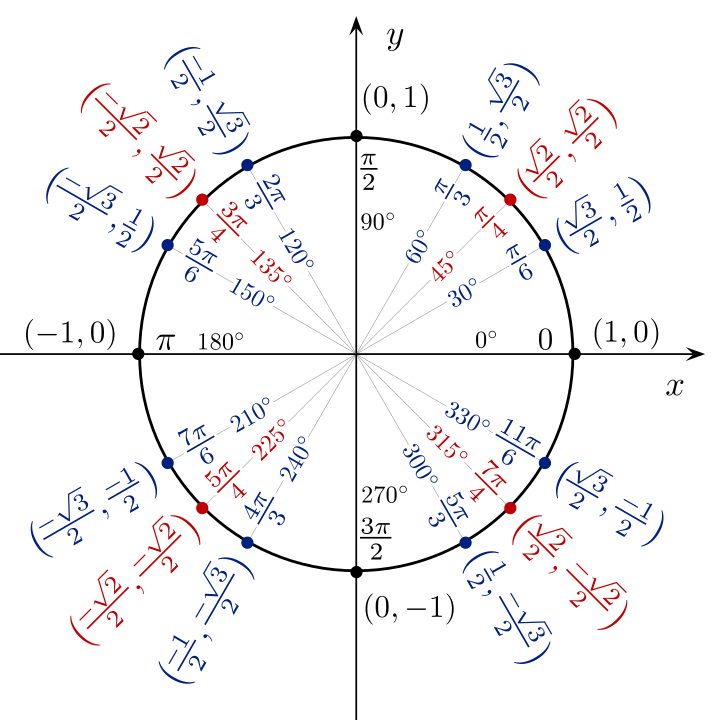
\includegraphics[scale=0.8]{vp}
\end{center}
Avant de passer à la sous-section suivante, démontrons une identité remarquable connue sous le nom de formule fondamentale de la trigonométrie. Celle-ci n'est en fait qu'une autre manière d'exprimer le théorème de Pythagore.
\begin{thé} [Formule fondamentale de la trigonométrie]~\\
$\forall x \in \rr$, on a :
$$\sin^2(x) + \cos^2(x) = 1$$
\end{thé}
\begin{proof}
Soit $x \in \rr$ et soit $A$ le point du cerlce trigonométrique associé à un angle orienté de mesure $x$. Soit $B$ le projeté orthogonal de $A$ sur l'axe des abscisses. \\
En fonction du quadrant dans lequel se trouve le point $A$, on peut représenter la situation par l'un des quatre dessins suivants :
\begin{enumerate}
\begin{multicols}{2}
\item ~\\ \begin{center} \begin{tikzpicture}[xmin=-1.3,xmax=1.1,ymin=-1.3,ymax=1.1, scale=1.5]{\axes}
\draw (0,0) circle (1);
\draw (0,0)node{$\bullet$};
\draw (0,0)node[below left]{O};
\draw (0:0)--(0:1);
\draw (0:0)--(60:1);
\draw [->](0.6,0) arc (0:60:0.6);
\draw (60:1) node {$\blackdiamond$}(30:0.8) node {$x$};
\draw (60:1)node[above right]{A};
\draw (0.5,0)node{$\bullet$};
\draw (0:0.5)node[below]{B};
\draw (60:1)--(0:0.5);
\end{tikzpicture}
\end{center}
\item ~\\ \begin{center} \begin{tikzpicture}[xmin=-1.3,xmax=1.1,ymin=-1.3,ymax=1.1, scale=1.5]{\axes}
\draw (0,0) circle (1);
\draw (0,0)node{$\bullet$};
\draw (0,0)node[below left]{O};
\draw (0:0)--(0:1);
\draw (0:0)--(150:1);
\draw [->](0.4,0) arc (0:150:0.4);
\draw (150:1) node {$\blackdiamond$}(75:0.5) node {$x$};
\draw (150:1)node[above left]{A};
\draw (-0.87,0)node{$\bullet$};
\draw (-0.87,0)node[below]{B};
\draw (-0.87,0)--(150:1);
\end{tikzpicture}
\end{center}
\item ~\\ \begin{center} \begin{tikzpicture}[xmin=-1.3,xmax=1.1,ymin=-1.3,ymax=1.1, scale=1.5]{\axes}
\draw (0,0) circle (1);
\draw (0,0)node{$\bullet$};
\draw (0,0)node[below left]{O};
\draw (0:0)--(0:1);
\draw (0:0)--(240:1);
\draw [->](0.4,0) arc (0:240:0.4);
\draw (240:1) node {$\blackdiamond$}(120:0.5) node {$x$};
\draw (240:1)node[below left]{A};
\draw (-0.5,0)node{$\bullet$};
\draw (-0.5,0)node[above left]{B};
\draw (-0.5,0)--(240:1);
\end{tikzpicture}
\end{center}
\item ~\\ \begin{center} \begin{tikzpicture}[xmin=-1.3,xmax=1.1,ymin=-1.3,ymax=1.1, scale=1.5]{\axes}
\draw (0,0) circle (1);
\draw (0,0)node{$\bullet$};
\draw (0,0)node[below left]{O};
\draw (0:0)--(0:1);
\draw (0:0)--(330:1);
\draw [->](0.4,0) arc (0:330:0.4);
\draw (330:1) node {$\blackdiamond$}(165:0.5) node {$x$};
\draw (330:1)node[below right]{A};
\draw (0.87,0)node{$\bullet$};
\draw (0.87,0)node[above]{B};
\draw (0.87,0)--(330:1);
\end{tikzpicture}
\end{center}
\end{multicols}
\end{enumerate}
Quel que soit le dessin qui convient, le triangle $\triangle OAB$ est rectangle en $B$. Par le théorème de Pythagore, on a :
$${|OA|}^{2} = {|OB|}^{2} + {|AB|}^{2}$$
Or, par définition des fonctions cosinus et sinus, les coordonnées du point $A$ sont $(\cos(x);\sin(x))$. Dès lors, on a $|OA|=1$ (car $[OA]$ est un rayon du cercle trigonométrique), $|OB|=|\cos(x)|$ et $|AB|=|\sin(x)|$. On a donc :
$${1}^{2} = {\left(|\cos(x)|\right)}^{2} + {\left(|\sin(x)|\right)}^{2}$$
En conclusion, puisque le carré de la valeur absolue d'un nombre réel est égal au carré de ce nombre réel :

$$1=\sin^2(x) + \cos^2(x)$$
\end{proof}
La formule fondamentale permet souvent de déterminer le cosinus d'un nombre à partir de son sinus et vice-versa. Donnons un exemple :
\begin{exe}
Soit $x=\frac{\pi}{12}$. Si je vous savez que $\cos(x)=\frac{\sqrt{6}+\sqrt{2}}{4}$, vous êtes à même de trouver la valeur exacte de $\sin(x)$. En effet, si $\cos(x)=\frac{\sqrt{6}+\sqrt{2}}{4}$, alors on a par la formule fondamentale :
$$1=\sin^2(x) + \cos^2(x)$$
$$1=\sin^2(x) + \left( \frac{\sqrt{6}+\sqrt{2}}{4} \right)^2$$
$$1=\sin^2(x) + \frac{6+2\sqrt{6}\sqrt{2}+2}{16}$$
$$\frac{16}{16}- \frac{6+2\sqrt{6}\sqrt{2}+2}{16}=\sin^2(x) $$
$$\frac{6-2\sqrt{6}\sqrt{2}+2}{16}=\sin^2(x) $$
$$\left( \frac{\sqrt{6}-\sqrt{2}}{4} \right)^2=\sin^2(x) $$
Comme $\frac{\pi}{12} \in [0;\frac{\pi}{4}]$, $\sin(x)$ est nécessairement positif. On en déduit que :
$$\frac{\sqrt{6}-\sqrt{2}}{4}=\sin(x) $$
\end{exe}
\newpage
\begin{exo}
En utilisant les propriétés élémentaires des fonctions cosinus et sinus ainsi que la proposition \ref{cossin}, calculer explicitement et sans calculatrice :
\begin{enumerate}
\begin{multicols}{2}
\item $\cos(\frac{\pi}{6})$
\item $\cos(\frac{3\pi}{4})$
\item $\cos(-\frac{7\pi}{6})$
\item $\cos(\frac{11\pi}{3})$
\item $\sin(-\frac{\pi}{4})$
\item $\sin(-\frac{5\pi}{2})$
\item $\sin(\frac{5\pi}{3})$
\item $\sin(-\frac{1000\pi}{6})$
\end{multicols}
\end{enumerate}
\end{exo}

\begin{exo}
~\\
\begin{enumerate}
\begin{multicols}{2}
\item $\cos(\frac{\pi}{6})=\frac{\sqrt{3}}{2}$
\item $\cos(\frac{3\pi}{4})=-\frac{\sqrt{2}}{2}$
\item $\cos(-\frac{7\pi}{6})=-\frac{\sqrt{3}}{2}$
\item $\cos(\frac{11\pi}{3})=\frac{1}{2}$
\item $\sin(-\frac{\pi}{4})=-\frac{\sqrt{2}}{2}$
\item $\sin(-\frac{5\pi}{2})=-1$
\item $\sin(\frac{5\pi}{3})=-\frac{\sqrt{3}}{2}$
\item $\sin(-\frac{1000\pi}{6})=-\frac{\sqrt{3}}{2}$
\end{multicols}
\end{enumerate}
\end{exo}

\begin{exo}
En utilisant les propriétés élémentaires des fonctions cosinus et sinus ainsi que la proposition \ref{cossin}, la formule fondamentale et sachant que $\cos(\frac{\pi}{8}) = \frac{\sqrt{2+\sqrt{2}}}{2}$, calculer explicitement et sans calculatrice :
\begin{enumerate}
\begin{multicols}{2}
\item $\sin(\frac{\pi}{8})$
\item $\cos(-\frac{5\pi}{8})$
\end{multicols}
\end{enumerate}
\end{exo}

\begin{solu}
~\\
\begin{enumerate}
\begin{multicols}{2}
\item $\sin(\frac{\pi}{8})=\frac{\sqrt{2-\sqrt{2}}}{2}$
\item $\cos(-\frac{5\pi}{8})=-\frac{\sqrt{2-\sqrt{2}}}{2}$
\end{multicols}
\end{enumerate}
\end{solu}

\newpage

\section{Définition des fonctions tangente et cotangente}

Il arrive fréquemment qu'il soit utile de pouvoir considérer le rapport du sinus d'un nombre par le cosinus de ce nombre ou le rapport du cosinus d'un nombre par le sinus de ce nombre. Pour que ces rapports fassent sens, il faut respectivement que le cosinus de ce nombre soit différent de $0$ et le sinus de ce nombre soit différent de $0$. Pour cette raison, les fonctions trigonométriques tangente et cotangente, définies comme ces deux rapports, n'ont pas comme domaine $\rr$ (il faut retirer l'ensemble des racines de la fonctions cosinus pour la fonction tangente et l'ensemble des racines de la fonction sinus pour la fonction cotangente).
\begin{déf}
La \emph{fonction tangente} est la fonction :
\begin{align*}
		\tan : \rr \backslash \{\frac{\pi}{2}+k\pi \in \rr ~|~k \in \zz\} &\to \rr \\
		x \mapsto& \frac{\sin(x)}{\cos(x)}
		\end{align*}
\end{déf}
\begin{déf}
La \emph{fonction cotangente} est la fonction :
\begin{align*}
		\cot : \rr \backslash \{k\pi \in \rr ~|~k \in \zz\} &\to \rr \\
		x \mapsto& \frac{\cos(x)}{\sin(x)}
		\end{align*}
\end{déf}
\begin{exe} ~\\
\begin{enumerate}
\item $\tan(\frac{\pi}{4}) = \frac{\sin(\frac{\pi}{4})}{\cos(\frac{\pi}{4})} = \frac{\frac{\sqrt{2}}{2}}{\frac{\sqrt{2}}{2}} = 1$
\item $\cot(\frac{\pi}{6}) = \frac{\cos(\frac{\pi}{6})}{\sin(\frac{\pi}{6})} = \frac{\frac{\sqrt{3}}{2}}{\frac{1}{2}} = \sqrt{3}$
		\end{enumerate}
\end{exe}
~\\
Les fonctions trigonométriques tangente et cotangente ont elles aussi une interprétation géométrique liée au cercle trigonométrique. Par exemple, pour la fonction tangente, pour $x \in ]0;\frac{\pi}{2}[$, si on désigne par $X$ le point du cercle trigonométrique associée à l'angle orienté de mesure $x$, si on note $A$ la projection orthogonale de $X$ sur l'axe des abscisses, $A'$ le point $(1;0)$ et $X'$ le point d'intersection de la droite $\overleftrightarrow{OX}$ avec la droite parallèle à l'axe des ordonnées passant par $A'$ :
\begin{center}
\begin{tikzpicture}[xmin=-1.3,xmax=1.1,ymin=-1.3,ymax=1.1, scale=3]{\axes}
\draw (0,0) circle (1);
\draw (1,-1.1)--(1,1.3);
\draw (1,0)node{$\bullet$};
\draw (0.8,0)node{$\bullet$};
\draw (1,0.73)node{$\bullet$};
\draw (0,0)node[below left]{O};
\draw (0:0)--(0:1);
\draw (0:0)--(36:2);
\draw (0.8,0)--(36:1);
\draw [->](0.4,0) arc (0:36:0.4);
\draw (36:1) node {$\blackdiamond$}(18:0.5) node {$x$};
\draw (36:1)node[above]{X};
\draw (0:1)node[below right]{A'};
\draw (0.8,0)node[below]{A};
\draw (1,0.73)node[right]{X'};
\end{tikzpicture}
\end{center}
On remarque alors que :
$$\tan(x) = \frac{\sin(x)}{\cos(x)} = \frac{|AX|}{|OA|}$$
Or, les triangles $\triangle OAX$ et $\triangle OA'X'$ sont semblables, on a donc par le théorème de Thalès :
$$\frac{|AX|}{|OA|} = \frac{|A'X'|}{|OA'|}$$
Comme $|OA'|=1$ (car $[OA']$ est un rayon du cercle trigonométrique), on a donc :
$$\tan(x) = |A'X'|$$
En conclusion, $\tan(x)$ est l'ordonnée du point $X'$. \\
~\\
Plus généralement, pour un $x \in \rr \backslash \{\frac{\pi}{2}+k\pi \in \rr ~|~k \in \zz\}$, on remarque (en utilisant le théorème de Thalès) que le nombre $\tan(x)$ est égal à l'ordonnée de l'intersection de la droite passant par l'origine et le point du cercle trigonométrique associé à un angle orienté de mesure $x$ avec la droite passant par le point $(1;0)$ et parallèlle à l'axe des ordonnées. \\
De même, pour tout $x \in \rr \backslash \{k\pi \in \rr ~|~k \in \zz\}$, on remarque pareillement (en utilisant le théorème de Thalès) que le nombre $\cot(x)$ est égal à l'abscisse de l'intersection de la droite passant par l'origine et le point du cercle trigonométrique associé à un angle orienté de mesure $x$ avec la droite passant par le point $(0;1)$ et parallèlle à l'axe des abscisses. \\
Pour résumer, visuellement :
\begin{center}
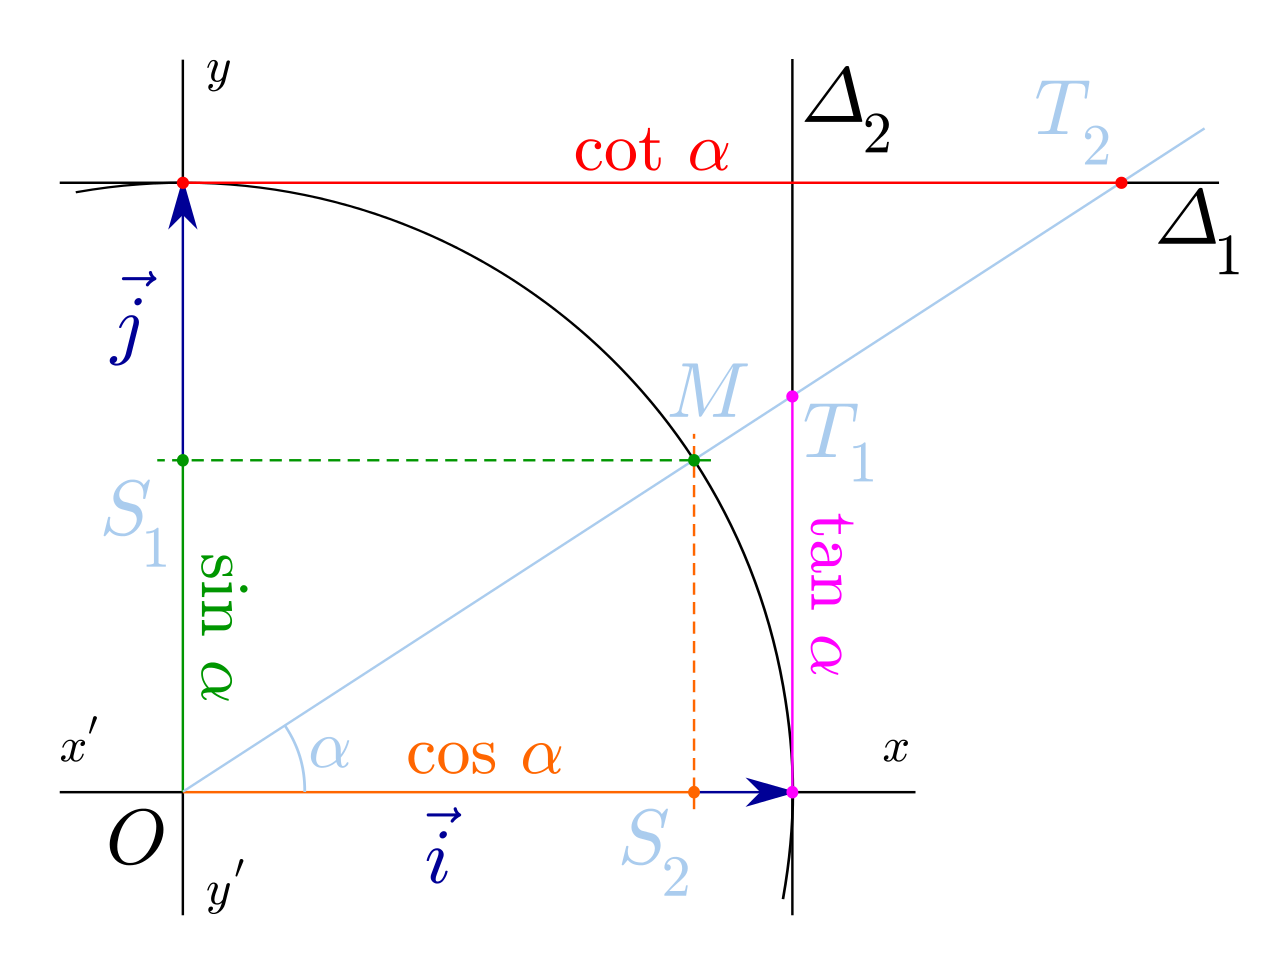
\includegraphics[scale=0.33]{ct}
\end{center}

\section{Valeurs particulières des fonctions tangente et cotangente} \label{sectionvptc}

\'Etant donné la définition de la fonction tangente et de la fonction cotangente, nous pouvons facilement calculer les nombres $\tan(0)$, $\tan(\frac{\pi}{6})$, $\tan(\frac{\pi}{4})$, $\tan(\frac{\pi}{3})$ et $\cot(\frac{\pi}{6})$, $\cot(\frac{\pi}{4})$, $\cot(\frac{\pi}{3})$, $\cot(\frac{\pi}{2})$. Nous obtenons alors un tableau similaire à celui que nous avions obtenu à la section \ref{sectionvp} pour les fonctions tangente et cotangente.
\begin{center}
\begin{Large}
\begin{tabular}{|c|c|c|c|c|c|}
  \hline
  $x$ & $0$ & $\frac{\pi}{6}$ & $\frac{\pi}{4}$ & $\frac{\pi}{3}$ & $\frac{\pi}{2}$\\
  \hline
  $\tan(x)$ & $0$ & $\frac{\sqrt{3}}{3}$ & $1$ & $\sqrt{3}$ & || \\
  \hline
  $\cot(x)$ & || & $\sqrt{3}$ & $1$ & $\frac{\sqrt{3}}{3}$ & $0$ \\
  \hline
\end{tabular}
\end{Large}
\end{center}
À nouveau, pour la plupart des autres valeurs de $x$, nous utiliserons dans ce cours la calculatrice pour estimer $\tan(x)$ et $\cot(x)$.

\section{Propriétés élémentaires des fonctions tangentes et cotangentes}

Les propriétés élémentaires des fonctions tangentes et cotangentes découlent directement de leur définition et des propriétés élémentaires des fonctions cosinus et sinus. \\
Par exemple, le fait que la fonction cosinus est paire et que la fonction sinus est impaire implique que la fonction tangente est impaire. En effet, pour tout $x \in \rr \backslash \{\frac{\pi}{2}+k\pi \in \rr ~|~k \in \zz\}$, on a :
$$\tan(-x) = \frac{\sin(-x)}{\cos(-x)} =\frac{-\sin(x)}{\cos(x)} = - \tan(x)$$
Nous laissons donc la démonstration de ces propriétés en exercice.
\begin{pro} [Propriétés élémentaires de la fonction tangente] ~\\
\begin{itemize}
\item Le domaine de définition de la fonction tangente est $\rr \backslash \{\frac{\pi}{2}+k\pi \in \rr ~|~k \in \zz\}$.
\item L'image de la fonction cosinus est $\rr$.
\item La fonction tangente est continue.
\item La fonction tengente est impaire.
\item La fonction cosinus est périodique de période $\pi$, c'est-à-dire que \\$\forall x \in \rr \backslash \{\frac{\pi}{2}+k\pi \in \rr ~|~k \in \zz\}$, on a : $$\tan(x) = \tan(x+\pi)$$
\item La fonction tangente est positive sur l'intervalle $[0;\frac{\pi}{2}[$, négative sur l'intervalle $]\frac{\pi}{2};\pi]$, positive sur l'intervalle $[\pi;\frac{3\pi}{2}[$, négative sur l'intervalle $]\frac{3\pi}{2};2\pi]$.
\item L'ensemble des racines de la fonction tangente est $\{k\pi \in \rr~|~k \in \zz \}$.
\item La fonction tangente n'a pas de point de maximum.
\item La fonction tangente n'a pas de point de minimum.
\end{itemize}
\end{pro}

\begin{pro} [Propriétés élémentaires de la fonction cotangente] ~\\
\begin{itemize}
\item Le domaine de définition de la fonction cotangente est $\rr \backslash \{k\pi \in \rr ~|~k \in \zz\}$.
\item L'image de la fonction cotangente est $\rr$.
\item La fonction cotangente est continue.
\item La fonction cotangente est impaire.
\item La fonction cotangente est périodique de période $\pi$, c'est-à-dire que \\$\forall x \in \rr \backslash \{k\pi \in \rr ~|~k \in \zz\}$, on a : $$\cot(x) = \cot(x+\pi)$$
\item La fonction cotangente est positive sur l'intervalle $]0;\frac{\pi}{2}]$, négative sur l'intervalle $[\frac{\pi}{2};\pi[$, positive sur l'intervalle $]\pi;\frac{3\pi}{2}]$, négative sur l'intervalle $[\frac{3\pi}{2};2\pi[$.
\item L'ensemble des racines de la fonction cotangente est $\{\frac{\pi}{2}+k\pi \in \rr~|~k \in \zz \}$.
\item La fonction cotangente n'a pas de point de maximum.
\item La fonction cotangente n'a pas de point de minimum.
\end{itemize}
\end{pro}
En utilisant les définitions et les propriétés élémentaires des fonctions tangente et cotangente, nous pouvons dessiner (approximativement) leur graphe :\\
\begin{itemize}
\begin{multicols}{2}
\item [Fonction tangente :]~\\
		\begin{tikzpicture}[xmin=-6,xmax=6,ymin=-6,ymax=6,scale=0.5]{\grille\axes}
\draw[thick,blue,samples=75] plot[domain=-6:1.40564-2*pi](\x,{tan(\x*(180/pi))});
\draw[thick,blue,samples=75] plot[domain=-1.40564-pi:1.40564-pi](\x,{tan(\x*(180/pi))});
\draw[thick,blue,samples=75] plot[domain=-1.40564:1.40564](\x,{tan(\x*(180/pi))});
\draw[thick,blue,samples=75] plot[domain=-1.40564+pi:1.40564+pi](\x,{tan(\x*(180/pi))});
\draw[thick,blue,samples=75] plot[domain=-1.40564+2*pi:6](\x,{tan(\x*(180/pi))});
		\end{tikzpicture}
~\\
\item [Fonction cotangente :]~\\
		\begin{tikzpicture}[xmin=-6,xmax=6,ymin=-6,ymax=6,scale=0.5]{\grille\axes}
\draw[thick,blue,samples=75] plot[domain=-6:2.97644-2*pi](\x,{cot(\x*(180/pi))});
\draw[thick,blue,samples=75] plot[domain=0.16515-pi:2.97644-pi](\x,{cot(\x*(180/pi))});
\draw[thick,blue,samples=75] plot[domain=0.16515:2.97644](\x,{cot(\x*(180/pi))});
\draw[thick,blue,samples=75] plot[domain=0.16515+pi:6](\x,{cot(\x*(180/pi))});
		\end{tikzpicture}
~\\
\end{multicols}
\end{itemize}
En exploitant la proposition \ref{cossin}, on démontre directement :
\begin{pro} \label{tancot}
$\forall x \in \rr \backslash \{k\frac{\pi}{2} \in \rr ~|~k \in \zz\}$, on a :
\begin{enumerate}
\item $\tan(\frac{\pi}{2} - x) = \cot(x)$ et $\cot(\frac{\pi}{2} - x) = \tan(x)$
\item $\tan(\frac{\pi}{2} + x) = -\cot(x)$ et $\cot(\frac{\pi}{2} + x) = -\tan(x)$
\item $\tan(\pi - x) = -\tan(x)$ et $\cot(\pi - x) = -\cot(x)$
\item $\tan(\pi + x) = \tan(x)$ et $\cot(\pi + x) = \cot(x)$
\end{enumerate}
\end{pro}
\`A nouveau, Les propriétés élémentaires des fonctions tangente et cotangente et la proposition \ref{tancot} permettent de calculer explicitement les nombres $\tan(x)$ et $\cot(x)$ pour de nombreuses valeurs de $x \in \rr$ à partir des valeurs particulières listées à la section \ref{sectionvptc}. Donnons quelques exemples :
\begin{exe}
\begin{enumerate}
\item $\tan(\frac{13\pi}{6}) = \tan(\frac{\pi}{6}+2\pi) = \tan(\frac{\pi}{6}) = \frac{\sqrt{3}}{3}$
\item $\cot(-\frac{\pi}{2}) = -\cot(\frac{\pi}{2}) = 0$
\item $\tan(\frac{2\pi}{3}) = \tan(\pi -\frac{\pi}{3}) =  -\tan(\frac{\pi}{3})=-\sqrt{3}$
\item $\cot(\frac{5\pi}{4}) = \cot(\pi +\frac{\pi}{4}) = \cot(\frac{\pi}{4})=1$
\end{enumerate}
\end{exe}
Avant de terminer cette section, démontrons l'équivalent de la  formule fondamentale de la trigonométrie pour les fonctions tangente et cotangente.
\begin{pro} \label{fftc} ~\\
$\forall x \in \rr \backslash \{\frac{\pi}{2}+k\pi \in \rr ~|~k \in \zz\}$, on a :
$$\tan^2(x) + 1 = \frac{1}{\cos^2(x)}$$
$\forall x \in \rr \backslash \{k\pi \in \rr ~|~k \in \zz\}$, on a :
$$1 + \cot^2(x) = \frac{1}{\sin^2(x)}$$
\end{pro}
\begin{proof}
Soit $x \in \rr \backslash \{\frac{\pi}{2}+k\pi \in \rr ~|~k \in \zz\}$. Par la formule fondamentale de la trigonométrie, on a :
$$\sin^2(x) + \cos^2(x)=1$$
Comme $x \notin  \{\frac{\pi}{2}+k\pi \in \rr ~|~k \in \zz\}$, on a $\cos(x) \neq 0$, on peut donc diviser l'identité par $\cos^2(x)$ :
$$\frac{\sin^2(x)}{\cos^2(x)} + \frac{\cos^2(x)}{\cos^2(x)}=\frac{1}{\cos^2(x)}$$
$$\tan^2(x) + 1 = \frac{1}{\cos^2(x)}$$
\`A présent, soit $x \in \rr \backslash \{k\pi \in \rr ~|~k \in \zz\}$. Par la formule fondamentale de la trigonométrie, on a :
$$\sin^2(x) + \cos^2(x)=1$$
Comme $x \notin  \{k\pi \in \rr ~|~k \in \zz\}$, on a $\sin(x) \neq 0$, on peut donc diviser l'identité par $\sin^2(x)$ :
$$\frac{\sin^2(x)}{\sin^2(x)} + \frac{\cos^2(x)}{\sin^2(x)}=\frac{1}{\sin^2(x)}$$
$$1 + \cot^2(x) = \frac{1}{\sin^2(x)}$$
\end{proof}
La proposition précédente permet souvent de déterminer le cosinus d'un nombre à partir de sa tangente et vice-versa ou le sinus d'un nombre à partir de sa cotangente et vice-versa. Donnons un exemple :
\begin{exe}
Soit $x=\frac{\pi}{12}$. Si vous savez que $\cos(x)=\frac{\sqrt{6}+\sqrt{2}}{4}$, vous êtes à même de trouver la valeur exacte de $\tan(x)$. En effet, si $\cos(x)=\frac{\sqrt{6}+\sqrt{2}}{4}$, alors on a par la proposition précédente :
$$\tan^2(x) + 1 = \frac{1}{\cos^2(x)}$$
$$\tan^2(x)= \frac{1}{\left( \frac{\sqrt{6}+\sqrt{2}}{4} \right)^2} -1$$
$$\tan^2(x)= \frac{1-\left( \frac{\sqrt{6}+\sqrt{2}}{4} \right)^2}{\left( \frac{\sqrt{6}+\sqrt{2}}{4} \right)^2}$$
$$\tan^2(x)= \frac{\frac{16}{16}- \frac{6+2\sqrt{6}\sqrt{2}+2}{16} }{\left( \frac{\sqrt{6}+\sqrt{2}}{4} \right)^2}$$
$$\tan^2(x)= \frac{\frac{6-2\sqrt{6}\sqrt{2}+2}{16} }{\left( \frac{\sqrt{6}+\sqrt{2}}{4} \right)^2}$$
$$\tan^2(x)= \frac{\left( \frac{\sqrt{6}-\sqrt{2}}{4} \right)^2}{\left( \frac{\sqrt{6}+\sqrt{2}}{4} \right)^2}$$
$$\tan^2(x)= \left( \frac{\sqrt{6}-\sqrt{2}}{\sqrt{6}+\sqrt{2}}\right)^2$$
$$\tan^2(x)= \left( \frac{\left(\sqrt{6}-\sqrt{2}\right)^2}{6-2}\right)^2$$
$$\tan^2(x)= \left( \frac{6-4\sqrt{3}+2}{4}\right)^2$$
$$\tan^2(x)= \left(2-\sqrt{3} \right)^2$$
Comme $\frac{\pi}{12} \in [0;\frac{\pi}{4}]$, $\tan(x)$ est nécessairement positif. On en déduit que :
$$\tan(x)= 2-\sqrt{3}$$
\end{exe}
\newpage
\begin{exo}
En utilisant les propriétés élémentaires des fonctions tangente et cotangente ainsi que la proposition \ref{tancot}, calculer explicitement et sans calculatrice :
\begin{enumerate}
\begin{multicols}{2}
\item $\tan(\frac{\pi}{6})$
\item $\tan(\frac{3\pi}{4})$
\item $\tan(-\frac{7\pi}{6})$
\item $\tan(\frac{11\pi}{3})$
\item $\cot(-\frac{\pi}{4})$
\item $\cot(-\frac{5\pi}{2})$
\item $\cot(\frac{5\pi}{3})$
\item $\cot(-\frac{1000\pi}{6})$
\end{multicols}
\end{enumerate}
\end{exo}

\begin{exo}
~\\
\begin{enumerate}
\begin{multicols}{2}
\item $\tan(\frac{\pi}{6})=\frac{\sqrt{3}}{3}$
\item $\tan(\frac{3\pi}{4})=-1$
\item $\tan(-\frac{7\pi}{6})=-\frac{\sqrt{3}}{3}$
\item $\tan(\frac{11\pi}{3})=-\sqrt{3}$
\item $\cot(-\frac{\pi}{4})=-1$
\item $\cot(-\frac{5\pi}{2})=0$
\item $\cot(\frac{5\pi}{3})=-\frac{\sqrt{3}}{3}$
\item $\cot(-\frac{1000\pi}{6})=\frac{\sqrt{3}}{3}$
\end{multicols}
\end{enumerate}
\end{exo}

\begin{exo}
En utilisant les propriétés élémentaires des fonctions cosinus et sinus ainsi que la proposition \ref{tangcot}, la proposition \ref{fftc} et sachant que $\cos(\frac{\pi}{8}) = \frac{\sqrt{2+\sqrt{2}}}{2}$, calculer explicitement et sans calculatrice :
\begin{enumerate}
\begin{multicols}{2}
\item $\tan(\frac{\pi}{8})$
\item $\cot(-\frac{5\pi}{8})$
\end{multicols}
\end{enumerate}
\end{exo}

\begin{solu}
~\\
\begin{enumerate}
\begin{multicols}{2}
\item $\tan(\frac{\pi}{8})=\sqrt{2}-1$
\item $\cot(-\frac{5\pi}{8})=\sqrt{2}-1$
\end{multicols}
\end{enumerate}
\end{solu}

\chapter{\'Equations trigonométriques simples}

Avant de s'attaquer à la modélisation de phénomènes périodiques et aux problèmes faisant intervenir des fonctions trigonométriques, nous allons nous entraîner à résoudre des équations trigonométriques simples. Plus précisément, nous allons nous entraîner à résoudre dans $\rr$ les équations qui peuvent se ramener sous la forme :
$$c.f(ax+b) + d =0$$
où $a,b,c,d \in \rr$ avec $a \neq 0$, $c \neq 0$ et $f$ est une des $4$ fonctions trigonométriques de référence que nous avons découvertes dans ce chapitre. \\
Nous allons d'abord procéder à une résolution générale, puis donner deux exemples de résolutions qui devraient couvrir la majeure partie des difficultés qu'il est possible de rencontrer.
\begin{rema}
La résolution d'une équation trigonométrique simple est très similaire à toutes les résolutions trigonométriques que vous avez déjà réalisées dans le passé. Fondamentalement, il n'y a aucune nouvelle difficulté, il faut juste avoir bien compris et connaître les définitions des fonctions trigonométriques ainsi que leurs propriétés élémentaires. \\
Une nouveauté qui surprendra peut-être certains d'entre vous est que les équations trigonométriques (simples), quand elles admettent des solutions, en admettent généralement une infinité (cela est dû à la périodicité des fonctions trigonométriques).
\end{rema}
Fixons $a,b,c,d \in \rr$ et $f$ une des quatre fonctions trigonométriques de référence (c'est-à-dire la fonction cosinus, la fonction sinus, la fonction tangente ou la fonction cotangente). Nous allons résoudre dans $\rr$ l'équation :
$$c.f(ax+b) + d =0$$
\begin{itemize}
\item [\'Etape $1$ :] Vérifier les conditions d'existence. Cela est important dans les cas où $f$ est la fonction tangente ou la fonction cotangente.
\item [\'Etape $2$ :] Comme $c \neq 0$, on peut alors diviser par $c$ et isoler la fonction trigonométrique :
$$f(ax+b)=-\frac{d}{c}$$
\item [\'Etape $3$ :] Vérifier si $-\frac{d}{c}$ appartient à l'image de $f$. Cela est important dans les cas où $f$ est la fonction cosinus ou sinus. Si ce n'est pas le cas, l'ensemble des solutions est l'ensemble vide.
\item [\'Etape $4$ :] Si $-\frac{d}{c}$ appartient à l'image de $f$, alors on cherche les nombres $y \in [0;2\pi[$ tels que :
$$f(y) = -\frac{d}{c}$$
Pour ce faire, on utilise les valeurs particulières connues des fonctions trigonométriques, ou bien on utilise la calculatrice\footnote{Pour trouver un nombre $y \in [0;\pi]$ tel que $\cos(y)$ est égal à un nombre entre $-1$ et $1$ donné, on utilise la fonction $\arccos$ de la calculatrice. Pour trouver un nombre $y \in [-\frac{\pi}{2};\frac{\pi}{2}]$ tel que $\sin(y)$ est égal à un nombre entre $-1$ et $1$ donné, on utilise la fonction $\arcsin$ de la calculatrice. Pour trouver un nombre $y \in ]-\frac{\pi}{2};\frac{\pi}{2}[$ tel que $\tan(y)$ est égal à un nombre réel donné, on utilise la fonction $\arctan$ de la calculatrice. Pour trouver un nombre $y \in ]0;\pi[$ tel que $\cot(y)$ est égal à un nombre réel donné, on utilise la fonction $\mathrm{arccot}$ de la calculatrice.}. \\
Remarque : faire un dessin d'un cercle trigonométrique peut aider pour cette étape.
\item [\'Etape $5$ :] Par périodicité des fonctions trigonométriques, si nous trouvons $y \in [0;2\pi[$ tels que :
$f(y) = -\frac{d}{c}$, alors pour tout $k \in \zz$, on a également $f(y+2k\pi) = -\frac{d}{c}$ (et même $f(y+k\pi) = -\frac{d}{c}$ si $f$ est la fonction tangente ou la fonction cotangente). Dès lors, pour tout $y \in [0;2\pi[$ tel que $f(y) = -\frac{d}{c}$ trouvé à l'étape précédente, il faut résoudre l'équation :
$$ax+b = y +2k\pi$$
pour tout $k \in \zz$. Ce qui n'est pas très difficile puisque $a \neq 0$ :
$$ax = y-b +2k\pi$$
$$x = \frac{y}{a}-\frac{b}{a} +k\frac{2\pi}{a}$$
L'ensemble des solutions est alors l'ensemble des nombres réels $x$ de cette forme, où $y$ est un des nombres compris entre $0$ compris et $2\pi$ non compris tel que $f(y) = -\frac{d}{c}$ trouvé à l'étape $4$ et $k$ est un nombre entier, duquel on a retiré les conditions d'existence de l'équation.
\end{itemize}
~\\
Donnons deux exemples.
\begin{exe}
Nous allons résoudre dans $\rr$ l'équation :
$$ \sin\left(2x+\frac{\pi}{5}\right)=\frac{\sqrt{3}}{2}$$
Tout d'abord, remarquons qu'il n'y a pas de condition d'existence à cette équation.  \\
La fonction trigonométrique a déjà été isolée. Cherchons donc les $y \in [0;2\pi[$ tels que :
$$\sin(y)=\frac{\sqrt{3}}{2}$$
Le nombre $\frac{\sqrt{3}}{2}$ est une valeur particulière de la fonction sinus : nous savons que $\sin(\frac{\pi}{3}) = \frac{\sqrt{3}}{2}$. \\
Mais $\frac{\sqrt{3}}{2}$ n'est pas le seul nombre $y \in [0;2\pi[$ tels que $\sin(y)=\frac{\sqrt{3}}{2}$ puisque $\forall z \in \rr$, on sait qu'on a $\sin(\pi - z) = \sin(z)$ (voir proposition \ref{cossin}). Dès lors, on a également $\sin(\frac{2\pi}{3})=\frac{\sqrt{3}}{2}$. Il n'y a pas d'autre $y \in [0;2\pi[$ tels que $\sin(y)=\frac{\sqrt{3}}{2}$ que $\frac{\pi}{3}$ et $\frac{2\pi}{3}$. \\
Dès lors, il nous faut résoudre dans $\rr$ deux équations :
$$2x+\frac{\pi}{5}=\frac{\pi}{3}+2k\pi$$
où $k \in \zz$, et :
$$2x+\frac{\pi}{5}=\frac{2\pi}{3}+2k\pi$$
où $k \in \zz$. \\
~\\
Commençons avec ;
$$2x+\frac{\pi}{5}=\frac{\pi}{3}+2k\pi$$
où $k \in \zz$. \\
On a :
$$2x+\frac{\pi}{5}=\frac{\pi}{3}+2k\pi$$
$$2x=\frac{\pi}{3}-\frac{\pi}{5}+2k\pi$$
$$x=\frac{\pi}{6}-\frac{\pi}{10}+k\pi$$
$$x=\frac{\pi}{15}+k\pi$$
\newpage
\`A présent, passons à :
$$2x+\frac{\pi}{5}=\frac{2\pi}{3}+2k\pi$$
où $k \in \zz$. \\
On a :
$$2x+\frac{\pi}{5}=\frac{2\pi}{3}+2k\pi$$
$$2x=\frac{2\pi}{3}-\frac{\pi}{5}+2k\pi$$
$$x=\frac{\pi}{3}-\frac{\pi}{10}+k\pi$$
$$x=\frac{7\pi}{30}+k\pi$$
~\\
En conclusion, puisqu'il n'y a pas de condition d'existence à l'équation, l'ensemble des solutions est :
$$\underset{k\in\zz}\bigcup \left\{\frac{\pi}{15}+k\pi ; \frac{7\pi}{30}+k\pi \right\} = \left\{\frac{\pi}{15}+k\pi ; \frac{7\pi}{30}+k\pi ~|~ k \in \zz \right\}$$
\end{exe}
~\\
\begin{exe}
Nous allons résoudre dans $\rr$ l'équation :
$$\frac{1}{2}\cot\left(-\frac{1}{3}x+\pi \right)+2=0$$
Tout d'abord, remarquons que pour cette équation fasse sens, il faut que $-\frac{1}{3}x+\pi$, c'est-à-dire que $-\frac{1}{3}x+\pi \neq k\pi$ où $k \in \zz$. Autrement dit :
$x$ doit être différent de $-3(k-1)\pi$ pour $k \in\zz$.  \\
Isolons la fonction trigonométrique :
$$\frac{1}{2}\cot\left(-\frac{1}{3}x+\pi \right)+2=0$$
$$\frac{1}{2}\cot\left(-\frac{1}{3}x+\pi \right)=-2$$
$$\cot\left(-\frac{1}{3}x+\pi \right)=-4$$
Maintenant que la fonction trigonométrique a été isolée, cherchons donc les $y \in [0;2\pi[$ tels que :
$$\cot(y)=-4$$
\newpage
Le nombre $-4$ n'est pas une valeur particulière de la fonction cotangente : la calculatrice nous donne une approximation d'un nombre $y$ entre $0$ et $\pi$ compris tel que $\cot(y)=-4$ : $y = \mathrm{arccot}(-4) \simeq 2,8966$. \\
Mais $\mathrm{arccot}(-4) \simeq 2,8966$ n'est pas le seul nombre $y \in [0;2\pi[$ tels que $\cot(y)=-4$ puisque $\forall z \in \rr \backslash \{k\pi \in \rr ~|~k \in \zz\}$, on sait qu'on a $\cot(\pi + z) = \cot(z)$ (voir proposition \ref{tancot}). Dès lors, on a également $\cot(\mathrm{arccot}(-4)+\pi)=-4$. Il n'y a pas d'autre $y \in [0;2\pi[$ tels que $\cot(y)=-4$ que $\mathrm{arccot}(-4) \simeq 2,8966$ et $\mathrm{arccot}(-4) + \pi \simeq 6,0382$. \\
Dès lors, il nous faut résoudre dans $\rr$ deux équations :
$$-\frac{1}{3}x+\pi=\mathrm{arccot}(-4)+2k\pi$$
où $k \in \zz$, et :
$$-\frac{1}{3}x+\pi=\mathrm{arccot}(-4) + \pi+2k\pi$$
où $k \in \zz$. \\
~\\
Commençons avec ;
$$-\frac{1}{3}x+\pi=\mathrm{arccot}(-4)+2k\pi$$
où $k \in \zz$. \\
On a :
$$-\frac{1}{3}x=\mathrm{arccot}(-4)-\pi+2k\pi$$
$$x=-3\mathrm{arccot}(-4)+3\pi -6k\pi \simeq 0,7349 -6k\pi$$
\`A présent, passons à :
$$-\frac{1}{3}x+\pi=\mathrm{arccot}(-4)+\pi+2k\pi$$
où $k \in \zz$. \\
On a :
$$-\frac{1}{3}x=\mathrm{arccot}(-4)+2k\pi$$
$$x=-3\mathrm{arccot}(-4)-6k\pi \simeq -8,6898 -6k\pi$$
\newpage
En conclusion, puisque les conditions d'existence n'impliquent pas ici qu'il faille rejeter certaines solutions, l'ensemble des solutions est :
$$\underset{k\in\zz}\bigcup \left\{-3\mathrm{arccot}(-4)+3\pi-6k\pi ; -3\mathrm{arccot}(-4)-6k\pi \right\} ={}$$
$$ \left\{-3\mathrm{arccot}(-4)+3\pi-6k\pi ; -3\mathrm{arccot}(-4)-6k\pi ~|~ k \in \zz \right\}$$
Avec approximations :
$$\underset{k\in\zz}\bigcup \left\{0,7349-6k\pi ; -8,6898-6k\pi \right\} = \left\{0,7349-6k\pi ; -8,6898-6k\pi ~|~ k \in \zz \right\}$$
\end{exe}
~\\
Résoudre des équations trigonométriques n'est pas compliqué, mais il est nécessaire de s'entraîner suffisamment pour que cela ne soit pas un frein à la compréhension pour la suite et fin du chapitre.
\begin{exo}
Résoudre dans $\rr$ sans calculatrice.
\begin{enumerate}
\begin{multicols}{2}
\item $\cos(x)=1$
\item $\cos(x)=2$
\item $\sin(x)-\frac{1}{2}=0$
\item $\sqrt{3}\tan(x)+1=0$
\item $4\cot(x+\frac{\pi}{3})-4=0$
\item $2\sqrt{2}\cos(x+\frac{\pi}{3})-2=0$
\item $\sqrt{3}\sin(2x+\frac{\pi}{6})=-\frac{3}{2}$
\item $\frac{1}{4}\sin(\frac{\pi}{17}x-13)-3=2$
\item $\tan(\pi x+\frac{3\pi}{4})=-1$
\item $\cot(-x+4)=-\sqrt{3}$
\end{multicols}
\end{enumerate}
\end{exo}

\begin{solu}
~\\
\begin{enumerate}
\item
$$S=\underset{k\in\zz}\bigcup \left\{0+2k\pi \right\} = \left\{2k\pi ~|~ k \in \zz \right\}$$
\item $$S=\emptyset$$
\item
$$S=\underset{k\in\zz}\bigcup \left\{\frac{\pi}{3}+2k\pi ; \frac{2\pi}{3}+2k\pi \right\} = \left\{\frac{\pi}{3}+2k\pi ; \frac{2\pi}{3}+2k\pi ~|~ k \in \zz \right\}$$
\item
$$S=\underset{k\in\zz}\bigcup \left\{\frac{5\pi}{6}+2k\pi ; \frac{11\pi}{6}+2k\pi \right\} = \left\{\frac{5\pi}{6}+k\pi ~|~ k \in \zz \right\}$$
\item
$$S=\underset{k\in\zz}\bigcup \left\{\frac{11\pi}{12}+2k\pi ; \frac{23\pi}{12}+2k\pi \right\} = \left\{\frac{11\pi}{12}+k\pi ~|~ k \in \zz \right\}$$
\item
$$S=\underset{k\in\zz}\bigcup \left\{\frac{17\pi}{12}+2k\pi ; \frac{23\pi}{12}+2k\pi \right\} = \left\{\frac{17\pi}{12}+2k\pi ; \frac{23\pi}{12}+2k\pi ~|~ k \in \zz \right\}$$
\item
$$S=\underset{k\in\zz}\bigcup \left\{\frac{3\pi}{4}+k\pi ; \frac{7\pi}{12}+k\pi \right\} = \left\{\frac{3\pi}{12}+k\pi ; \frac{7\pi}{12}+k\pi ~|~ k \in \zz \right\}$$
\item $$S=\emptyset$$
\item $$S=\zz$$
\item $$S=\underset{k\in\zz}\bigcup \left\{\frac{\pi}{6}+4-\pi -k\pi \right\} = \left\{\frac{\pi}{6}+4+k\pi ~|~ k \in \zz \right\}$$
\end{enumerate}
\end{solu}

\begin{exo}
Résoudre dans $\rr$ avec calculatrice.
\begin{enumerate}
\begin{multicols}{2}
\item $\cos(x)=\frac{\sqrt{3}}{3}$
\item $2\tan(3x+\pi)-\frac{\pi}{2}=0$
\end{multicols}
\end{enumerate}
\end{exo}

\begin{solu}
Avec approximations :
\begin{enumerate}
\item $$S=\underset{k\in\zz}\bigcup \left\{0,95532+2k\pi ; 5,32787+2k\pi \right\} = \left\{0,95532+2k\pi ; 5,32787+2k\pi ~|~ k \in \zz \right\}$$
\item $2\tan(3x+\pi)-\frac{\pi}{2}=0$
$$\underset{k\in\zz}\bigcup \left\{0,22192+k\frac{\pi}{3} \right\} = \left\{0,22192+k\frac{\pi}{3} ~|~ k \in \zz \right\}$$
\end{enumerate}
\end{solu}

\chapter{Phénomènes périodiques}

\section{Modélisation de phénomènes périodiques}

Nous sommes enfin en mesure d'aborder un des buts principaux de ce chapitre : la modélisation de phénomènes périodiques\footnote{Un phénomène périodique est un phénomène qui se répète dans le temps.} à l'aide des fonctions trigonométriques. \\
L'année prochaine, vous utiliserez ce type de modélisation dans votre cours de sciences, en particulier en physique lorsque vous discuterez des ondes. \\
Commençons avec un exemple.

\begin{exe}
Nous allons modéliser la situation suivante : supposons que je joue au yoyo. \`A l'instant $t=0$, le jouet se trouve dans ma main qui se situe à une hauteur de $1$m du sol et je commence à jouer avec. Sachant que la corde du yoyo est d'une longueur de $1$m et que j'entretiens le mouvement du yoyo de sorte que celui-ci effectue un aller-retour toutes les $3$s, sommes-nous capable de modéliser le mouvement du yoyo, c'est-à-dire (cans ce cas-ci) déterminer une fonction qui donne la hauteur du yoyo par rapport au sol en fonction du temps ? \\
~~\\
Puisque le mouvement du yoyo est périodique, une fonction qui donnerait la hauteur de celui-ci par rapport au sol en fonction du temps devrait être périodique (au sens mathématique). Heureusement, nous connaissons à présent des exemples de fonctions périodiques : les fonctions trigonométriques. Puisque la heuteur du yoyo oscille entre une hauteur maximale (de $1$m) et une hauteur minimale (de $0$m) de façon continue, il semble que les fonctions $\sin$ et $\cos$ seraient adaptées comme choix de fonction pour notre modélisation. Choisissons en une des deux : la fonction sinus.\footnote{Si elle ne convient pas, nous réessayerons avec la fonction cosinus.}\newpage
La fonction sinus elle-même modélise-t-elle correctement la hauteur du yoyo par rapport au sol en fonction du temps ?
\begin{center}
\begin{align*}
		f_1 : \rr &\to \rr \\
		t \mapsto& \sin(t)
		\end{align*}
\end{center}
\begin{center}
		\begin{tikzpicture}[xmin=-10,xmax=10,ymin=-2,ymax=2,scale=0.7]{\grille\axes}
		\draw[thick,blue,samples=100] plot[domain=-10:10](\x,{sin(\x*(180/pi))});
		\end{tikzpicture}
	\end{center}
Malheureusement, non. Puisque la hauteur intermédiaire du yoyo, celle qui se situe à mi-chemin entre la hauteur maximale ($1$m) et la hauteur minimale ($0$m) est $0,5$m et non $0$m, il nous faut adapter cette fonction. Comme la moyenne du maximum et du minimum de la fonction sinus est $0$, ajoutons la constante $0,5$ à la fonction $f_1$.
\begin{center}
\begin{align*}
		f_2 : \rr &\to \rr \\
		t \mapsto& \sin(t)+0,5 
		\end{align*}
\end{center}
\begin{center}
		\begin{tikzpicture}[xmin=-10,xmax=10,ymin=-2,ymax=2,scale=0.7]{\grille\axes}
		\draw[thick,blue,samples=100] plot[domain=-10:10](\x,{0.5+sin(\x*(180/pi))});
		\end{tikzpicture}
	\end{center}
La fonction $f_2$ modélise-t-elle correctement la hauteur du yoyo par rapport au sol en fonction du temps ? \`A nouveau, non, il nous faut encore la modifier quelque peu. En effet, l'écart entre le maximum et le minimum de $f_2$ est de $2$ et non de $1$ alors que l'écart entre la hauteur maximale du yoyo et sa hauteur minimale est de $1$m. Pour remédier à ce problème, multiplions la par $0,5$, de sorte que l'écart entre le maximum et le minimum de la fonction devienne $2.0,5=1$.
\begin{center}
\begin{align*}
		f_3 : \rr &\to \rr \\
		t \mapsto& 0,5 \sin(t) +0,5
		\end{align*}
\end{center}
\begin{center}
		\begin{tikzpicture}[xmin=-10,xmax=10,ymin=-2,ymax=2,scale=0.7]{\grille\axes}
		\draw[thick,blue,samples=100] plot[domain=-10:10](\x,{0.5+0.5*sin(\x*(180/pi))});
		\end{tikzpicture}
	\end{center}
Nous n'avons pas encore fini : en effet, à l'instant $t=0$, le yoyo se trouve à une hauteur de $1$m et non de $f_3 (0) = 0,5$m. Pour adapter $f_3$, nous avons alors deux possibilités : soit remplacer la fonction sinus dans l'expression de $f_3$ par la fonction cosinus (étant donné que $\cos (0)=1$), soit ajouter $\frac{\pi}{2}$ à l'argument de la fonction sinus dans l'expression de $f_3$. Choisissons cette deuxième possibilité.
\begin{center}
\begin{align*}
		f_4 : \rr &\to \rr \\
		t \mapsto& 0,5 \sin\left(t+\frac{\pi}{2}\right) +0,5
		\end{align*}
\end{center}
\begin{center}
		\begin{tikzpicture}[xmin=-10,xmax=10,ymin=-2,ymax=2,scale=0.7]{\grille\axes}
		\draw[thick,blue,samples=100] plot[domain=-10:10](\x,{0.5+0.5*sin(\x*(180/pi)+90)});
		\end{tikzpicture}
	\end{center}
Nous y sommes presque : il nous faut encore tenir compte du fait que le yoyo réalise un aller-retour complet toutes les $3$s. Or, la période de $f_4$ est de $2\pi$ et non de $3$. Multiplions donc l'argument $t$ par $\frac{2\pi}{3}$ dans l'expression de $f_4$.
\begin{center}
\begin{align*}
		f : \rr &\to \rr \\
		t \mapsto& 0,5 \sin\left(\frac{2\pi}{3}t+\frac{\pi}{2}\right) +0,5
		\end{align*}
\end{center}
\begin{center}
		\begin{tikzpicture}[xmin=-10,xmax=10,ymin=-2,ymax=2,scale=0.7]{\grille\axes}
		\draw[thick,blue,samples=100] plot[domain=-10:10](\x,{0.5+0.5*sin((2*pi/3)*\x*(180/pi)+90)});
		\end{tikzpicture}
	\end{center}
Vérifions si cette dernière fonction $f$ modélise bien notre phénomène périodique :
\begin{itemize}
\item $f(0)=0,5 \sin(0+\frac{\pi}{2}) +0,5=1$ : la hauteur du yoyo en $t=0$ est bien de $1$m.
\item Le maximum de $f$ est $1$ et le minimum de $f$ est $0$ : le hauteur du yoyo oscille entre $1$m et $0$m.
\item $f$ est périodique de période $3$ : le yoyo met $3$s pour réaliser un aller-retour complet.
\end{itemize}
Notre fonction $f$ modélise donc bien le phénomène observé. Comme nous pouvons le constater avec cet exemple, la fonction sinus joue un rôle majeur dans la modélisation de ce phénomène périodique qu'est le mouvement (entretenu) d'un yoyo. Il est en fait possible de justifier à partir d'expériences et de théories scientifiques que la fonction sinus est même plus que satisfaisante pour la modélisation de ce phénomène périodique (et de bien d'autres) : elle est idéale. Malheureusement, nous n'avons pas l'occasion de présenter ces justifications dans le cadre de ce cours.
\begin{rema}
Le choix que nous avons réalisé pour modifier la fonction $f_3$ de telle sorte qu'elle tienne compte de la hauteur du yoyo à l'instant $t=0$ est arbitraire et nous aurions pu d'ailleurs choisir comme point de départ la fonction cosinus plutôt que la fonction sinus et arriver à un résultat équivalent. En effet, puisque pour tout $t \in \rr$, on a $\sin(t + \frac{\pi}{2}) = \cos(t)$, notre fonction $f$ est telle que pour tout $t \in \rr$, $f(t) = 0,5 \sin(\frac{2\pi}{3}t+\frac{\pi}{2}) +0,5 = 0,5 \cos(\frac{2\pi}{3}t) +0,5$. Néanmoins, par convention, on choisit généralement d'utiliser la fonction sinus pour modéliser des phénomènes périodiques.
\end{rema}
\begin{rema}
Si nous souhaitons être tout à fait rigoureux, la fonction $f$ ne modélise pas encore le phénomène observé. En effet, le mouvement du yoyo commence à l'instant $t=0$ et doit bien se terminer à un certain moment (je ne suis pas capable d'entretenir le mouvement du yoyo éternellement). Si je suppose par exemple que je joue au yoyo pendant $18$ secondes, je devrais restreindre la fonction $f$ sur $[0;18]$ pour obtenir une fonction qui modélise réellement la hauteur du yoyo en fonction du temps, pour tout instant $t$ compris entre le début et la fin de l'observation.

%\begin{center}
%\begin{align*}
%		f : [0;20] &\to \rr \\
%		t \mapsto& 0,5 \sin\left(\frac{2\pi}{3}t+\frac{\pi}{2}\right) +0,5
%		\end{align*}
%\end{center}
%\begin{center}
%		\begin{tikzpicture}[xmin=-0.5,xmax=18.5,ymin=-2,ymax=2,scale=0.7]{\grille\axes}
%		\draw[thick,blue,samples=100] plot[domain=-0:18](\x,{0.5+0.5*sin((2*pi/3)*\x*(180/pi)+90)});
%		\draw[thick,blue] (0,1)node{$\bullet$};
%		\draw[thick,blue] (18,1)node{$\bullet$};
%		\end{tikzpicture}
%	\end{center}
\end{rema}
\end{exe}
\newpage
La démarche de modélisation que nous avons réalisée pour cet exemple n'est pas propre à celui-ci. Plus généralement, pour modéliser un phénomène périodique, on utilise souvent une fonction de la forme\footnote{Nous pourrions remplacer la fonction sinus par la fonction cosinus, cela fonctionnerait également. Par convention, on choisit généralement la fonction sinus.} :
\begin{center}
\begin{align*}
		f : \rr &\to \rr \\
		t \mapsto& A \sin(\omega t+\phi) +b
		\end{align*}
\end{center}
où $A,b,\omega,\phi$ sont quatre paramètres réels avec $A \neq 0$ et $\omega \neq 0$. Dans un tel contexte de modélisation d'un phénomène périodique, ceux-ci portent un nom et ont une interprétation physique :~~\\
\begin{itemize}
\item $A$ est \emph{l'amplitude}. C'est un paramètre qui dépend de la spatialité du phénomène que l'on souhaite modéliser et est égal à la moitié de l'écart entre la plus grande et la plus petite valeur prises par la quantité modélisée. L'amplitude correspond souvent à \og l'intensité \fg{} du phénomène.
\item $b$ est le \emph{décalage vertical}. C'est un paramètre qui dépend de la spatialité du phénomène que l'on souhaite modéliser et est égal à la moyenne de la plus grande et de la plus petite valeur prises par la quantité modélisée. Le décalage vertical correspond souvent au \og niveau de base \fg{} du phénomène.
\item $\omega$ est la \emph{vitesse angulaire}. C'est un paramètre qui dépend de la temporalité du phénomène que l'on souhaite modéliser. La vitesse angulaire correspond parfois à la vitesse à laquelle un objet observé tourne sur lui-même. Plus généralement, la vitesse angulaire correspond à la \og vitesse \fg{} du phénomène.
\item $\phi$ est le \emph{déphasage}. C'est un paramètre qui dépend de la temporalité du phénomène que l'on souhaite modéliser. Le déphasage a plusieurs interprétations possibles en fonction du contexte. Il correspond par exemple parfois au délai avant le début de l'observation du phénomène modélisé.
\end{itemize}~~\\
De plus, on peut définir deux notions propres au phénomène modélisé à partir de ces paramètres, qui ont elles aussi une interprétation physique.
\newpage
\begin{déf}
La \emph{période} du phénomène périodique modélisé est le nombre $$T = \frac{2\pi}{|\omega|}$$
La période correspond à la durée de temps qui s'écoule avant que le phénomène ne se répète.
\end{déf}
\begin{déf}
La \emph{fréquence} du phénomène périodique modélisé est le nombre $$f = \frac{1}{T}$$
La fréquence correspond au nombre de répétitions du phénomène par unité de temps.
\end{déf}
Dans notre exemple du yoyo, la période était une des données et la fréquence était de $\frac{1}{3}$s. \\
L'année prochaine, vous verrez que la période et la fréquence sont des notions très utiles lorsqu'on étudie les ondes.

\section{Problèmes faisant intervenir les fonctions trigonométriques}

Maintenant que nous sommes capables de modéliser des phénomènes périodiques à l'aide des fonctions trigonométriques et nous avons appris à résoudre des équations trigonométriques simples, nous avons tous les outils nécessaires pour répondre à des problèmes par rapport auxquels nous étions autrefois démunis. Donnons deux exemples (faits en classe).

\begin{exe}
Approximons l'orbite de la Terre autour du Soleil comme un cercle dans le plan de l'écliptique et supposons que la distance Terre-Soleil est constante et est égale à une unité astronomique, c'est-à-dire environ $150000000$km.
\begin{enumerate}
\item Quelle distance la Terre parcourt-elle (avec comme point de repère le Soleil) en $1$ mois ?
\item Quelle est la distance qui sépare les positions de la Terre (avec comme point de repère le Soleil) de 23 août et du 23 décembre ?
\end{enumerate}
\end{exe}

\begin{exe}
Soit une masse suspendue à un ressort de $50$cm attaché verticalement à une poutre se trouvant à $2$m au dessus du sol. Ecartée de sa position d'équilibre d'une distance de $1$cm pour être ensuite relâchée, la masse se met à osciller au rythme d'une oscillation toutes les $\frac{\pi}{4} \simeq 0,785$ seconde. On néglige les forces de frottement de l'air. On demande :
\begin{enumerate}
\item De donner une fonction qui exprime la distance de la masse par rapport au sol (en cm) en fonction du temps (en s) et de dessiner son graphe.
\item De donner une fonction qui exprime la distance (en cm) de la masse par rapport à la poutre en fonction du temps (en s) et de dessiner son graphe.
\item De donner la distance de la masse par rapport au sol $\frac{9\pi}{8} \simeq 3,534$s après avoir laché la masse.
\item De déterminer après combien de temps la masse atteindra sa position la plus haute pour la première fois.
\item De calculer le nombre de fois que la masse passera par sa position la plus basse sur un intervalle de temps de $10$s.
\end{enumerate}
\end{exe}

Voici d'autres exercices pour s'entraîner :

\begin{exo}
La température d'une pièce oscille entre $10$ degrés Celsius et $20$ degrés Celsius. La température minimale est atteinte une seule fois par jour, vers $3$h. La température maximale est atteinte une seule fois par jour, vers $15$h. On demande de :
\begin{enumerate}
\item Donner une fonction qui modélise la température (en degré Celsius) de la pièce en fonction du temps (en heure).
\item Grâce à cette fonction, prédire exactement à quels moments de la journée la température de la pièce sera de $15$ degrés Celsius.
\item En utilisant le graphe de cette fonction, déterminer graphiquement et approximativement à quels moments de la journée la température de la pièce sera de $18$ degrés Celsius.
\end{enumerate}
\end{exo}
\begin{solu}
\begin{enumerate}
\item 
\begin{align*}
		f : \rr &\to \rr \\
		t \mapsto& 5 \sin(\frac{2\pi}{24} t+15.\frac{2\pi}{24}) +15
		\end{align*}
\item Vers $9$h et vers $21$h.
\item Un peu avant $11$h$30$ et un peu après $18$h$30$.
\end{enumerate}
\end{solu}

\begin{exo}
Un bateau à roues dont $\frac{3}{4}$ des roues ($\frac{3}{4}$ des diamètres verticaux des roues) sont immergées fait fonctionner ses moteurs de telle sorte que ses roues réalisent un tour complet sur elles-mêmes toutes les $2$ minutes. Ces roues ont un rayon de $3$m. Si un marin doit effectuer une réparation d'urgence sur une des roues alors que celle-ci tourne, combien a-t-il de temps (en seconde) pour travailler sur un point externe précis de cette roue avant que cette partie de la roue ne soit à nouveau immergée ? Quid si les roues sont immergées à $93,3$\%.\footnote{Question bonus : une des données est en fait inutile pour la résolution du problème. Laquelle et pourquoi ?}
\end{exo}
\begin{solu}
$40$ secondes et (approximativement) $20$ secondes.
\end{solu}

\chapter{Exercices supplémentaires}

\section{Série 1 : énoncés}

\begin{benumerate}[14pt]

\item Résous dans $\rr$.
\begin{benumerate}[3pt]
\begin{multicols}{2}
\item $\d \cos x = 0,5$
\item $\d \tan x = -\frac{\sqrt{3}}{3}$
\item $\d \sin 2x = 0,45931$
\item $\d \sin (9x-1)=1,2$
\item $\d 2\cos^2 x = 1$
\item $\d \tan^2 3x - 1 = 0$
\end{multicols}
\end{benumerate}

\item Recherche le domaine de définition maximal et l'ensemble des racines de la fonction $f$.
\begin{align*}
f : ? \to& \rr \\
x \mapsto& \frac{1}{2\cos (3x+1)}
\end{align*}

\item Aurore et Pierre observent l'envol d'une montgolfière à bord de laquelle se trouve l'un de leurs copains. Aurore et Pierre se sont placés à 100~m du point d'envol et la montgolfière s'est élevée verticalement. Lorsque le bas de la nacelle est à 50~m d'altitude, ils l'aperçoivent sous un angle $\alpha$. La ballon poursuit son ascension verticale. De combien de mètres a-t-il progressés lorsqu'ils voient la bas de la nacelle sous un angle $2\alpha$ ? On suppose que les yeux des observateurs sont situés à 1,6~m du sol.

\item Précise l'amplitude, le déphasage, la période, la fréquence et le décalage vertical pour chacune des fonctions suivantes.
\begin{benumerate}[3pt]
\item $\d f(t)=\sin\left(\frac{2\pi}{5}t\right)$
\item $\d f(t) = 2\sin\left(\frac{\pi}{12}(t-1)\right)+3$
\item $\d f(t) = \frac{1}{2}\cos\left(\pi t - \frac{\pi}{4}\right)-1$
\end{benumerate}

\item La grande roue de Walibi a un diamètre de 50~m, son point le plus haut est situé à 55~m et elle effectue un tour en 120~secondes. Quelle est l'expression de la fonction qui permet de décrire la distance au sol d'un point de cette grande roue ?

\item Explicite les différentes étapes permettant de construire les graphiques des fonctions suivantes au départ du graphique de $\sin~t$ ou de $\cos~t$.
\begin{benumerate}
\item $\d f(t)=2\sin\left(4t-\frac{\pi}{3}\right)+1$
\item $\d f(t)=\frac{2}{3}\cos\left(2t+\frac{3\pi}{4}\right)$
\end{benumerate}

\item L'ensemble des relevés de température au cours d'une journée se prête parfois à une modélisation par une fonction de la forme $f(t)=A\sin(\omega t + \varphi)+b$, dans laquelle $t$ est le temps exprimé en heures et $f(t)$ la température en degrés Celsius. Dans ce cas, minuit correspond à $t=0$ et on suppose que la température décroit dans les premières heures de relevés.
\begin{benumerate}
\item Quelle est la fonction qui modélise l'évolution de la température d'une journée durant laquelle le maximum est de 10 ${}^{\degree}$C et le minimum, atteint à 3h, est de -2 ${}^{\degree}$C ?
\item Quelle était la température à minuit ?
\item Pendant combien de temps a-t-il gelé ?
\item Pendant quelles périodes de la journée a-t-on eu une température supérieure à 8 ${}^{\degree}$C ?
\end{benumerate}

\end{benumerate}

\section{Série 1 : solutions}

\begin{benumerate}[10pt]

\item \begin{benumerate}[5pt]
\item $\d S = \left\{ \frac{\pi}{3}+2k\pi ~;~ -\frac{\pi}{3}+2k\pi~|~k\in\zz \right\}$
\item CE : $\d x \neq \frac{\pi}{2}+k\pi ~(k\in\zz)$,\quad $\d S = \left\{ -\frac{\pi}{6}+k\pi~|~ k \in \zz\right\}$
\item $\d S = \left\{ 0,239+k\pi~;~1,332+k\pi ~|~k\in\zz \right\}$
\item $\d S = \emptyset$
\item $\d S = \left\{ \frac{\pi}{4}+\frac{k\pi}{2}~|~k\in\zz\right\}$
\item CE : $\d x \neq \frac{\pi}{6}+\frac{k\pi}{3} ~(k\in\zz)$,\quad $\d S = \left\{ \frac{\pi}{12}+\frac{k\pi}{6}~|~k\in\zz \right\}$
\end{benumerate}

\item $\d dom~f = \rr \backslash\left\{ \frac{2\pi}{9}+\frac{2k\pi}{3} ~;~ -\frac{2\pi}{9}+\frac{2k\pi}{3}~|~k\in\zz \right\}$ et la fonction n'admet pas de racine.

\item Le ballon s'est élevé de 78 mètres.

\renewcommand{\arraystretch}{1.2}

\item \begin{tabular}{|c|c|c|c|c|c|}
\hline
 & Amplitude & Déphasage & Période & Fréquence & Décalage vertical \\
\hline
\textbf{(a)} & $1$ & $0$ & $5$ & $0,2$ & $0$ \\
\hline 
\textbf{(b)} & $2$ & $1$ & $24$ & $\d \frac{1}{24}$ & $3$ \\
\hline
\textbf{(c)} & $\d \frac{1}{2}$ & $\d \frac{1}{4}$ & $2$ & $\d \frac{1}{2}$ & $-1$ \\
\hline
\end{tabular}

\item La fonction est $\d f(t)=30+25\sin\left(\frac{\pi}{60}t+\varphi\right)$ ; $\varphi$ est la phase d'origine, elle dépend de la position du point observé au début du mouvement (non donné dans l'énoncé).

\item \begin{benumerate}[5pt]
\item Déphasage : $\d 4t-\frac{\pi}{3}=0$ donc $\d t =\frac{\pi}{12}$.
\begin{benumerate}
\item On trace le graphe de $\sin t$ ;
\item on translate ce graphe de $\d \frac{\pi}{3}$ unités vers la droite ;
\item on divise toutes les abscisses par $4$ ;
\item on multiplie toutes les ordonnées par $2$ ;
\item on translate le graphe d'$1$ unité vers le haut.
\end{benumerate}
\item Déphasage : $\d 2t+\frac{3\pi}{4}=0$ donc $\d t = -\frac{3\pi}{8}$
\begin{benumerate}
\item On trace le graphe de $\cos t$ ;
\item on translate ce graphe de $\d \frac{3\pi}{4}$ unités vers la gauche ;
\item on divise toutes les abscisses par $2$ ;
\item on multiplie toutes les ordonnées par $\d \frac{2}{3}$.
\end{benumerate}
\end{benumerate}

\item \begin{benumerate}[5pt]
\item $\d f(t)=6\sin\left(\frac{\pi t}{12}+\frac{5\pi}{4}\right)+4$
\item La température est de $-0,24$ ${}^{\degree}$C.
\item Il a gelé pendant 6h 26min sur cette journée (entre 0h et 6h13 et entre 23h47 et 24h). Cela se repère sur un graphique très précis de la fonction, par exemple tracé sur Geogebra.
\item Il a fait plus de 8 ${}^{\degree}$C entre 11h47 et 18h13. Cela se repère sur un graphique très précis de la fonction, par exemple tracé sur Geogebra.
\end{benumerate}
\end{benumerate}

\newpage

\section{Série 2 : énoncés}

\begin{benumerate}[14pt]

\item Calcule sans calculatrice sachant que $\sin(1)\simeq$ 0,84, $\cos(1)\simeq$ 0,54 et $\tan(1)\simeq$ 1,56 :
\begin{multicols}{3}
\begin{benumerate}
\item $\d\sin\left(\frac{5\pi}{6}\right)=~?$
\item $\d\cos\left(-\frac{\pi}{6}\right)=~?$
\item $\d\tan\left(\frac{5\pi}{3}\right)=~?$
\item $\d\sin\left(\frac{11\pi}{6}\right)=~?$
\item $\d\cos\left(-\frac{5\pi}{6}\right)=~?$
\item $\d\tan\left(\frac{-3\pi}{4}\right)=~?$
\item $\d\sin\left(\pi-1\right)\simeq ~? $
\item $\d\cos\left(-\frac{\pi}{2}+1\right)\simeq ~?$
\item $\d\cot\left(\frac{\pi}{2}-1\right)\simeq ~?$
\item $\d\sin\left(\frac{3\pi}{2}-1\right)\simeq v$
\item $\d\cos\left(-\pi+1\right)\simeq ~?$
\item $\d\tan\left(-1\right)\simeq ~?$
\end{benumerate}
\end{multicols}

\item Résous dans $\rr$.
\begin{benumerate}[3pt]
\begin{multicols}{2}
\item $\d \cos x =$ 0,5
\item $\d \tan x = -\frac{\sqrt{3}}{3}$
\item $\d \sin 2x =$ 0,45931
\item $\d \sin (9x-1)=$ 1,2
\end{multicols}
\end{benumerate}

\item Recherche le domaine de définition et l'ensemble des racines de la fonction $\d f(x)=\frac{1}{2\cos 3x+1}$.

\item Décris en termes d'intervalles de réels les parties de cercle trigonométrique données dans les figures suivantes :

\begin{center}
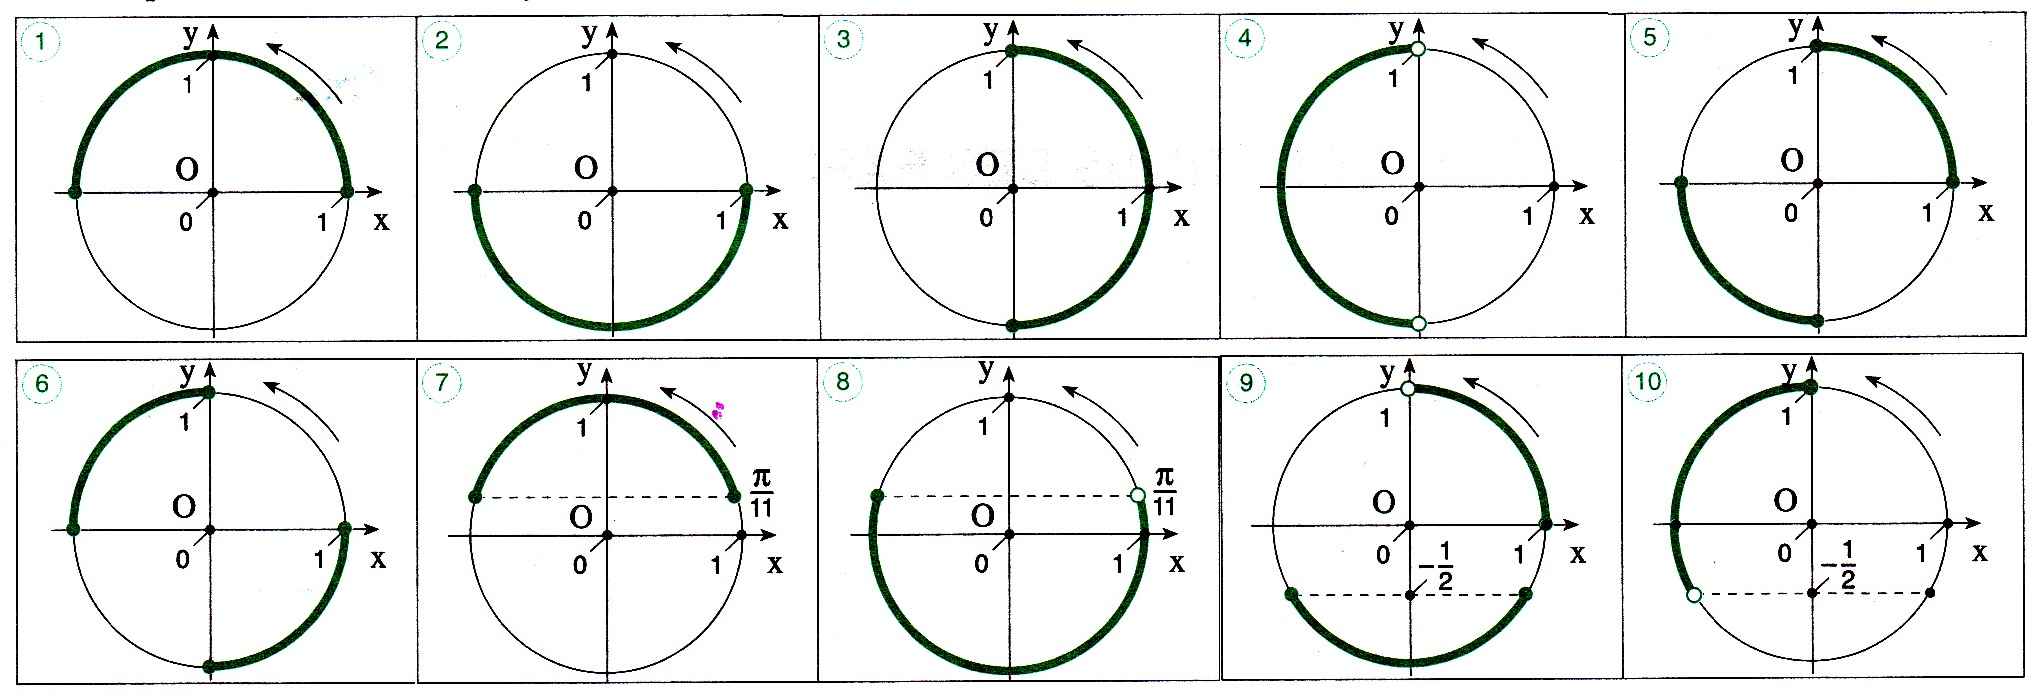
\includegraphics[height=5.1cm]{ex_intervalles.jpg}
\end{center}

\item Détermine le domaine de définition maximal et l'ensemble des racines de la fonction $f$ :
\begin{benumerate}[5pt]
\begin{multicols}{3}
\item $\d f(x) = \sqrt{\sin x}$
\item $\d f(x) = \sqrt{\tan x + 1}$
\item $\d f(x) = \sqrt{2\cos 3x -1}$
\end{multicols}
\end{benumerate}

\end{benumerate}

\newpage
\section{Série 2 : solutions}

\begin{benumerate}

\item \begin{multicols}{3}
\begin{benumerate}
\item $\frac{1}{2}$
\item $\frac{\sqrt{3}}{2}$
\item $-\sqrt{3}$
\item $-\frac{1}{2}$
\item $-\frac{\sqrt{3}}{2}$
\item $1$
\item 0,84
\item 0,84
\item 1,56
\item $-$0,54
\item $-$0,54
\item $-$1,56
\end{benumerate}
\end{multicols}

\item 
\begin{enumerate}
\item $\d S = \left\{\frac{\pi}{3}+2k\pi ~ ; ~ -\frac{\pi}{3}+2k\pi ~ \middle| ~ k\in \zz \right\}$
\item CE : $\d x \neq \frac{\pi}{2}+k\pi~(k\in\zz)$, $\d S = \left\{ -\frac{\pi}{6}+k\pi ~ \middle| ~ k \in \zz \right\}$
\item $\d S = \left\{ \text{0,239}+k\pi ~ ; ~ \text{1,332}+k\pi ~\middle|~k \in \zz \right\}$
\item $\d S = \emptyset$
\end{enumerate}

\item
\begin{benumerate}
\item $\dom f=\rr\backslash\left\{\frac{2\pi}{9}+\frac{2k\pi}{3}~;~-\frac{2\pi}{9}+\frac{2k\pi}{3}~\middle|~k\in\zz\right\}$ ; racines : aucune
\end{benumerate}

\item 
\begin{benumerate}
\item[(1)] $\d I = \underset{k\in\zz}\cup \left[2k\pi~;~\pi+2k\pi\right]$
\item[(2)] $\d I = \underset{k\in\zz}\cup \left[-\pi+2k\pi~;~2k\pi\right]$
\item[(3)] $\d I = \underset{k\in\zz}\cup \left[-\frac{\pi}{2}+2k\pi~;~\frac{\pi}{2}+2k\pi\right]$
\item[(4)] $\d I = \underset{k\in\zz}\cup \left]\frac{\pi}{2}+2k\pi~;~\frac{3\pi}{2}+2k\pi\right[$
\item[(5)] $\d I = \underset{k\in\zz}\cup \left[k\pi~;~\frac{\pi}{2}+k\pi\right]$
\item[(6)] $\d I = \underset{k\in\zz}\cup \left[-\frac{\pi}{2}+k\pi~;~k\pi\right]$
\item[(7)] $\d I = \underset{k\in\zz}\cup \left[\frac{\pi}{11}+2k\pi~;~\frac{10\pi}{11}+2k\pi\right]$
\item[(8)] $\d I = \underset{k\in\zz}\cup \left[-\frac{12\pi}{11}+2k\pi~;~\frac{\pi}{11}+2k\pi\right[$
\item[(9)] $\d I = \underset{k\in\zz}\cup \left(\left[2k\pi~;~\frac{\pi}{2}+2k\pi\right[\cup\left[\frac{7\pi}{6}+2k\pi~;~\frac{11\pi}{6}+2k\pi\right]\right)$
\item[(10)] $\d I = \underset{k\in\zz}\cup \left[\frac{\pi}{2}+2k\pi~;~\frac{7\pi}{6}+2k\pi\right[$
\end{benumerate}

\item
\begin{benumerate}
\item $\dom f = \d \underset{k\in\zz}\cup \left[2k\pi ~;~ \pi+2k\pi \right]$, racines = $\left\{ k\pi ~|~ k\in\zz \right\}$
\item dom = $\d \underset{k\in\zz}\cup \left[ -\frac{\pi}{4} + k\pi ~;~ \frac{\pi}{2} + k\pi \right[$, racines = $\d \left\{ -\frac{\pi}{4}+k\pi ~\middle|~ k\in\zz \right\}$
\item dom = $\d \underset{k\in\zz}\cup \left[ -\frac{\pi}{9}+\frac{2k\pi}{3} ~;~ \frac{\pi}{9}+\frac{2k\pi}{3} \right]$, racines = $\d \left\{ -\frac{\pi}{9}+\frac{2k\pi}{3} ~;~ \frac{\pi}{9}+\frac{2k\pi}{3} ~\middle|~ k\in\zz \right\}$
\end{benumerate}

\end{benumerate}

\chapter{Annexe}

Depuis cette année, des résultats importants portants sur les fonctions trigonométriques ne font plus partie du programme de mathématiques 4 heures/semaine, alors même qu'il s'agit de résultats importants dont aura probablement besoin votre professeur de physique l'année prochaine. Pour cette raison, nous allons lister ceux-ci (sans démonstration) et il est vivement conseillé de les parcourir au moins une fois en préparation du cours de physique de l'année prochaine.

\begin{pro} [Dérivabilité des fonctions trigonométriques]~\\
Les fonctions trigonométriques :
\begin{enumerate}
	\begin{multicols}{2}
		\item \begin{align*}
		f : \rr &\to \rr \\
		x \mapsto& \cos(x)
		\end{align*}
		\item \begin{align*}
		g : \rr &\to \rr \\
		x \mapsto& \sin(x)
		\end{align*}
		\item \begin{align*}
		h : \rr \backslash \{\frac{\pi}{2}+k\pi \in \rr& ~|~ k \in \zz \} \to \rr \\
		x \mapsto& \tan(x)
		\end{align*}
\item \begin{align*}
		l : \rr \backslash \{\pi+k\pi \in \rr& ~|~ k \in \zz \} \to \rr \\
		x \mapsto& \cot(x)
		\end{align*}
	\end{multicols}
\end{enumerate}
sont dérivables et on a :
\begin{enumerate}
	\begin{multicols}{2}
		\item \begin{align*}
		\forall x & \in \rr :\\
		f'(x)&=-\sin(x)
		\end{align*}
		\item \begin{align*}
		\forall x & \in \rr :\\
		g'(x)&=\cos(x)
		\end{align*}
		\item \begin{align*}
		\forall x \in \rr \backslash \{\frac{\pi}{2}&+k\pi \in \rr ~|~ k \in \zz \} :\\
		h'(x)=&\frac{1}{\cos^2(x)}
		\end{align*}
\item \begin{align*}
		\forall x \in \rr \backslash \{\pi&+k\pi \in \rr ~|~ k \in \zz \} :\\
		l'(x)=&-\frac{1}{\sin^2(x)}
		\end{align*}
	\end{multicols}
\end{enumerate}
\end{pro}

\begin{pro} [Formules d'addition pour les fonctions cosinus et sinus]~\\
Pour tout $a,b \in \rr$, on a :
\begin{enumerate}
\item $\cos(a-b) = \cos(a)\cos(b) + \sin(a)\sin(b)$
\item $\cos(a+b) = \cos(a)\cos(b) - \sin(a)\sin(b)$
\item $\sin(a-b) = \sin(a)\cos(b) - \cos(a)\sin(b)$
\item $\sin(a+b) = \sin(a)\cos(b) + \cos(a)\sin(b)$
\end{enumerate}
\end{pro}

\begin{pro} [Formules d'addition pour la fonction tangente]~\\
Pour tout $a,b \in \rr \backslash \{\frac{\pi}{2}+k\pi \in \rr~|~k \in \zz\}$ tels que $a+b \notin \rr \backslash \{\frac{\pi}{2}+k\pi \in \rr~|~k \in \zz\}$, on a :
\begin{enumerate}
\item $\tan(a-b) = \frac{\tan(a)-\tan(b)}{1+\tan(a)\tan(b)}$
\item $\tan(a+b) = \frac{\tan(a)+\tan(b)}{1-\tan(a)\tan(b)}$
\end{enumerate}
\end{pro}

\begin{pro} [Formules d'addition pour les fonctions cosinus et sinus] ~\\
Pour tout $a \in \rr$, on a :
\begin{enumerate}
\item $\cos(2a) = \cos^2(a) - \sin^2(a)$
\item $\sin(2a) = 2\sin(a)\cos(a)$
\end{enumerate}
\end{pro}

\begin{pro} [Formules d'addition pour la fonction tangente]~\\
Pour tout $a \in \rr \backslash \{\frac{\pi}{2}+k\pi \in \rr~|~k \in \zz\}$ tel que $2a \notin \rr \backslash \{\frac{\pi}{2}+k\pi \in \rr~|~k \in \zz\}$, on a :
\begin{enumerate}
\item $\tan(2a) = \frac{2\tan(a)}{1-\tan^2(a)}$
\end{enumerate}
\end{pro}

\begin{pro} [Formules de Carnot (formules de linéarisation)]~\\
Pour tout $a \in \rr$, on a :
\begin{enumerate}
\item $\cos^2(a) = \frac{1}{2}(1+\cos(2a))$
\item $\sin^2(a) = \frac{1}{2}(1-\cos(2a))$
\end{enumerate}
\end{pro}

\begin{pro} [Formules de Simpson (formules de factorisation)]~\\
Pour tout $p,q \in \rr$, on a :
\begin{enumerate}
\item $\sin(p)+\sin(q) = 2 \sin(\frac{p+q}{2})\cos(\frac{p-q}{2})$
\item $\sin(p)-\sin(q) = 2 \cos(\frac{p+q}{2})\sin(\frac{p-q}{2})$
\item $\cos(p)+\cos(q) = 2 \cos(\frac{p+q}{2})\cos(\frac{p-q}{2})$
\item $\cos(p)-\cos(q) = -2 \sin(\frac{p+q}{2})\sin(\frac{p-q}{2})$
\end{enumerate}
\end{pro}

\begin{pro} [Formule en $\tan(\frac{x}{2}$]~\\
Pour tout $x \in \rr$, si $x \notin \{\pi+2k\pi \in \rr~|~k \in \zz \}$, on a :
\begin{enumerate}
\item $\cos(x) = \frac{1-\tan^2(\frac{x}{2})}{1+\tan^2(\frac{x}{2})}$
\item $\sin(x) = \frac{2\tan(\frac{x}{2})}{1+\tan^2(\frac{x}{2})}$
\item Si de plus $x \notin \{\frac{\pi}{2}+k\pi \in \rr~|~k \in \zz \}$ : $\tan(x) = \frac{2\tan(\frac{x}{2})}{1-\tan^2(\frac{x}{2})}$
\end{enumerate}
\end{pro}
\end{document}
